\documentclass{article}


\usepackage[round]{natbib}
\usepackage{amsmath,amssymb,amsthm,bm,enumerate,mathrsfs,mathtools}
\usepackage{latexsym,color,verbatim,multirow}
\usepackage{graphicx}
\usepackage{caption}
\usepackage{subcaption}
\usepackage{tikz}
\usepackage{geometry}
\usetikzlibrary{shapes,arrows}
\tikzstyle{block} = [rectangle, draw, fill=white!20,
    text width=7em, text centered, rounded corners, minimum height=4em]
\tikzstyle{title} = [text width=7em, text centered, font=\bfseries]
\tikzstyle{line} = [draw, -latex']


\usepackage{mycommands}

\begin{document}

\newtheorem{theorem}{Theorem}
\newtheorem{corollary}[theorem]{Corollary}
\newtheorem{lemma}[theorem]{Lemma}
\newtheorem{observation}[theorem]{Observation}
\newtheorem{proposition}[theorem]{Proposition}
\newtheorem{definition}[theorem]{Definition}
\newtheorem{claim}[theorem]{Claim}
\newtheorem{fact}[theorem]{Fact}
\newtheorem{assumption}[theorem]{Assumption}
\newtheorem{model}[theorem]{Model}

\theoremstyle{definition}
\newtheorem{example}{Example}

\newcommand{\cM}{\mathcal{M}}
\newcommand{\cH}{\mathcal{H}}
\newcommand{\cD}{\mathcal{D}}
\newcommand{\FDR}{\textnormal{FDR}}
\newcommand{\FCR}{\textnormal{FCR}}
\newcommand{\crt}{\phi}
\newcommand{\M}{\mathcal{M}}
\newcommand{\cY}{\mathcal{Y}}
\newcommand{\cX}{\mathcal{X}}
\newcommand{\cV}{\mathcal{V}}
\newcommand{\bX}{\mathbf{X}}
\newcommand{\x}{\mathbf{x}}
\newcommand{\Gv}{\;\;\big|\;\;}
%\newcommand{\cP}{\mathcal{P}}
\newcommand{\proj}{\cP}
\newcommand{\pow}{\text{Pow}}
\newcommand{\sF}{\mathscr{F}}
\newcommand{\cF}{\mathcal{F}}
\newcommand{\sC}{\mathscr{C}}
\newcommand{\hJ}{\widehat{J}}
\newcommand{\bH}{\mathbf{H}}
\newcommand{\bM}{\mathbf{M}}
\newcommand{\tM}{\widetilde{M}}
\newcommand{\tE}{\widetilde{E}}
\newcommand{\tV}{\widetilde{V}}
\newcommand{\tR}{\widetilde{R}}
\newcommand{\tL}{\widetilde{L}}
\newcommand{\hk}{\hat{k}}
\newcommand{\hr}{\hat{r}}
\newcommand{\cN}{\mathcal{N}}
\newcommand{\cJ}{\mathcal{J}}
\newcommand{\leqAS}{\overset{\textrm{a.s.}}{\leq}}
\newcommand{\Err}{\mathcal{E}}


\newcommand*\mystrut{\vrule width0pt height0pt depth1.5ex\relax}
\newcommand{\underlabel}{\underbracket[1pt][.5pt]{\mystrut \quad\;\; \sub \quad\;\; }}
\newcommand{\JTcomment}[1]{{\color{blue}{(JT: \bf \sc #1) }}}
\newcommand{\WFcomment}[1]{{\color{red}{(WF: \bf \sc #1) }}}
\newcommand{\RTcomment}[1]{{\color{green}{(RT: \bf \sc #1) }}}

\title{Adaptive Sequential Model Selection}
\author{William Fithian, Jonathan Taylor, Rob Tibshirani, and Ryan Tibshirani}
\maketitle

\begin{abstract}
  Many model selection algorithms produce a ``path'' of fits specifying a sequence of increasingly complex models. Given such a sequence and the data used to produce them, we consider the problem of choosing the least complex model that is not falsified by the data. Extending the selected-model tests of \citet{fithian2014optimal}, we construct $p$-values for each step in the path, accounting for the fact that the model path is determined adaptively using the data. In the case of linear regression, our $p$-values improve on the power of the spacings test of \citet{taylor2014exact}, often dramatically.
  We also show that the selected models test  bears a close relationship to parametric bootstrap sampling, 

To choose a model we feed the resulting $p$-values as inputs into sequential stopping rules proposed by \citet{gsell2013sequential} and \citet{li2015accumulation}, achieving adaptive control of the familywise error rate or false discovery rate. These stopping rules assume that the single-step null $p$-values are independent of each other and of the non-null $p$-values, a condition that is not satisfied by the $p$-values of \citet{taylor2014exact}. We derive intuitive and general conditions for independence and show that our proposed constructions yield independent $p$-values.
\end{abstract}


\section{Introduction}
\label{sec:introduction}
Many model selection procedures produce  a sequence of increasingly complex models. Often our goal is to choose the simplest model that is not falsified by the available data.
In other words, we seek  the index of the smallest adequate model ---  the smallest model that cannot be falsified given available evidence.
Examples of such model selection procedures include  forward stepwise linear regression, least angle regression (LAR) and  the ever-active path in $\ell_!$-regularized models .
All of these were studied in \citet{taylor2014exact}. Another, different, example is principal components analysis in which we try to determine the correct rank of the
covariance matrix. This problem was studied in \citet{choi2014selecting}.

A natural way carry out this model selection is as follows: we compute a set  of sequential p-values   at each step of the path of models and then feed them into a stopping rule
that provides guaranteed control of the false discovery rate (FDR) or a similar quantity. Recently  \citet{gsell2013sequential} and \citet{li2015accumulation} proposed sequential stopping rules of this kind.
Both sets of rules require that once we have reached the correct model in our path, the p-values in subsequent steps are uniform (or sub-uniform)
and independent.
In this paper we develop a theoretical framework for the construction of sequential p-values  that are both (sub)-uniform and independent under the correct model,
and show how to construct them  in forward stepwise regression, LAR and the ever-active path in $\ell_1$-regularized models.
In the former case, the test is simply a sequential selective version the max-$t$ test of ~\citet{buja2014}, based on the theory developed \citet{fithian2014optimal}.

Table \ref{tab:diab} shows an example: using the diabetes data taken from \cite{LARS}.
These data consist of  observations on $442$ patients, with the response of interest being a quantitative measure of disease progression one year after baseline.
There are ten baseline variables---age, sex, body-mass index, average blood pressure,
and six blood serum measurements---plus quadratic terms, giving a total of 64 features.


\begin{table}[ht]
\centering
\begin{tabular}{rrrrr}
  \hline\\
 Step& Predictor& Naive pvalue& Saturated pvalue& Max-t pvalue\cr
  \hline\\
1 & 3& 0.00 & 0.00 & 0.00 \\ 
  2 & 9 & 0.00 & 0.00 & 0.00 \\ 
  3 & 4 & 0.00 & \color{red}{0.05} & 0.00 \\ 
  4 & 20 & 0.00 & 0.33 & 0.01 \\ 
  5 & 37 & 0.00 & 0.76 & 0.05 \\ 
  6 & 7 & 0.00 & 0.25 & 0.05 \\ 
  7 & 2 & 0.00 & 0.00 & 0.00 \\ 
  8 & 19 & 0.02 & 0.03 & \color{red}{0.37} \\ 
  9 & 11 & 0.11 & 0.55 & 0.95 \\ 
  10 & 52 & 0.21 & 0.91 & 0.92 \\ 
  11 & 57 & 0.05 & 0.37 & 0.21 \\ 
  12 & 24 & 0.22 & 0.15 & 0.00 \\ 
  13 & 5 & 0.18 & 0.07 & 0.10 \\ 
  14 & 49 & 0.16 & 0.97 & 0.75 \\ 
  15 & 30& 0.21 & 0.15 & 0.05 \\ 
  16 & 46 & \color{red}{0.16} & 0.05 & 0.53 \\ 
  17 & 59 & 0.27 & 0.45 & 0.68 \\ 
  18 & 33 & 0.12 & 0.71 & 0.80 \\ 
  19 & 62 & 0.08 & 0.40 & 0.48 \\ 
  20 & 27 & 0.17 & 0.60 & 0.50 \\ 
   \hline\\
\end{tabular}
\caption[tab:diab]{\em Forward stepwise regression for the diabetes data: naive p-values from forward stepwise regression, 
p-values from the ``saturated'' model, and the ``max-t'' p-values that are presented in this paper. The red annotation indicates the stopping step
prescribed by {\tt forwardStop}. For the max-t p-values, this gives exact FDR control at the 10\% level.}
\label{tab:diab}
\end{table}
The table shows the naive p-values from forward stepwise regression, that do not account for the selection, as well as the
p-values from the ``saturated'' model, and the ``max-t'' p-values that are presented in this paper.
The latter two sets of p-values test someone different hypotheses:  the p-values from the saturated model test whether the partial regression of the predictor just added is zero,
what we call the ``incremental null''
In contrast, the max-t pvalues test whether the current model is adequate, that is, all predictors not in the model  have coefficients equal to zero,
the ``complete null''. (The issue of what hypothesis to test is discussed in section \ref{sec:whichnull}.)
Now it turns out that the max-t test is often more powerful that the saturated model test, and importantly, the max-t pvalues are exactly
independent after we reach the point the model sequence when the complete null is true. This independence means that we can apply
sequential FDR exact stopping rules, such as ``forwardStop'' (\citet{gsell2013sequential}). When applied to the max-t pvalues at FDR 0.10, {\tt forwardStop}
suggested stopping at step 8. In constant, the saturated lvalues gave stopping a point of 3, with no guarantee of FDR control
due to the lack of independence of the p-values.

An outline of this paper is as follows:
In Section \ref{sec:genericSetting} we setup the problem and give some important definitions. In Section \ref{sec:sequential} we review recently proposed methods for
testing ordered hypothesis using from a sequence of p-values. These method require that the p-values be uniform and independent under the null, and we derive general conditions
to ensure this property. In Section \ref{sec:singleStep}  we  show how to construct valid selective $p$-values for a single step in the path and derive the max-t test
for  forward stepwise regression and the Next-$\lambda$ test for the lasso. Section \ref{sec:computation}  describes our computational strategy for estimating the p-values using accept-reject and hit and run sampling. We also relate the method to parametric bootstrap sampling. We provide a simulation study in Section \ref{sec:sparseReg} and briefly discuss applications of our framework to
principal components analysis in section\ref{sec:pca}. The paper ends with a Discussion.

%\begin{example}[Forward-Stepwise Linear Regression]
 % \citet{taylor2014exact}
%end{example}

%\begin{example}[The LARS Algorithm in Regression]
%  \citet{taylor2014exact}
%\end{example}

%\begin{example}[Ever-Active Path in $\ell_1$-Regularized Methods]
 % \citet{taylor2014exact}
%\end{example}

%\begin{example}[Principal Components Analysis]
%  As a second motivating example, consider model selection for   principal components analysis. In that case we are given a data matrix $X \in \R^{n\times d}$, with which we form a sample %covariance matrix
%\[
%S = \frac{1}{n-1} \sum_{i=1}^n(x_i - \bar x)^2
%\]
%The first $d$ principal component loadings are the first $d$ eigenvectors of $S$, which call $u_1,\ldots, u_d$. These induce a sequence of nested Wishart models:
%\[
%M_0 \sub M_1 \sub \cdots \sub M_d
%\]
%n which
%\begin{equation}
 % M_k:\; (n-1) S \sim W_d\left(\lambda_0 I_d + \sum_{i=1}^k     \lambda_i u_i u_i', \;\;\; n-1\right).
%\end{equation}
%This problem was studied in \citet{choi2014selecting}.
%\end{example}

\section{Notation and Problem Setting}
\label{sec:genericSetting}

More generically, we observe data $Y \in \cY$, with unknown sampling distribution $F$. We then use $Y$ to generate an adaptive sequence of $d$ nested models
\[
M_0(Y) \sub M_1(Y) \sub \cdots \sub M_d(Y) \sub M_\infty.
\]
\WFcomment{should probably end with $M_{d-1}(Y)$. need to fix this throughout paper.}
\RTcomment{Will- be more specific here---   A parametric model  with
  specified nonzero support?}
\WFcomment{Not necessarily. As far as I can tell, there's no need to restrict ourselves in either case. $Y\sim U[0,\theta]$ is a perfectly good model; so is a Cox proportional hazards model.}

By ``model,'' we mean a family of probability distributions for $Y$. Without loss of generality, we can take $M_\infty$ as the union of all models under consideration. We will use the notation $M_{0:k}$ to denote the sequence of the first $k$ models.

Define the {\em completion index} $k_0(Y) = \min\{k:\; F \in M_k(Y)\}$, the index of the first correct model. By construction, $F\in M_k \iff k \geq k_0$. Our goal is to examine the data and output a {\em stopping rule}, i.e. an estimator $\hk(Y)$ of $k_0$. We consider $M_k$ to be ``rejected'' if $k < \hat k$, and ``accepted'' otherwise. Thus $\hk$ is the number of models we rejected, while $k_0$ is the number that we should have rejected. 

The number of type I errors is $V=(\hk-k_0)_+$, while the number of type II errors is $(k_0-\hk)_+$. Depending on the context we might want to control the familywise error rate (FWER) $\P(V>0)$, the false discovery rate (FDR) $\E[V/(\hk \vee 1)]$, or another error rate given by the expectation of some loss function $g$:
\begin{equation}\label{eq:errRate}
\Err_F(\hk(\cdot), g) = \E_F\left[ g\left(\hk(Y), k_0(Y)\right)\right]
\end{equation}

We will assume that for each candidate model $M$ there is a minimal sufficient statistic $T(Y; \,M)$, and write
\[
T_k(Y) = T(Y; M_k(Y)).
\]

First suppose that we have single step p-values for testing
\[
H_{k}:\; F\in M_{k-1}(Y)
\]
against the alternative that $F\in M_\infty\setminus M_{k-1}$. The $p$-values must account for the fact that the models are chosen adaptively. 
\citet{gsell2013sequential} and \citet{li2015accumulation} propose stopping rules that operate on the sequence $p_{1:d}$. These stopping rules provably control certain error rates, provided that the null $p$-values are mutually independent and independent of the non-null $p$-values. 
We review these methods in Section~\ref{sec:sequential} .

Hence the task is to  construct sequential p-values which satisfy the above requirements, and we do this in Section \ref{sec:singleStep}.
We also discuss general conditions under which single-step $p$-values are independent.


\subsection{Linear Regression}

Most of our examples will focus on the important and familiar problem of adaptively selecting a set of predictors in linear regression models. In this problem, we observe a random response $Y\in \R^n$ as well as a fixed design matrix $X\in \R^{n \times p}$, whose columns correspond to candidate predictors. For each {\em active set} $E \sub \{1,\ldots,p\}$, there is a corresponding candidate model
\[
M(E):\; Y \sim \cN( X_E\beta, \sigma^2 I_n),
\]
which is a subset of the {\em full model}
\[
M_\infty:\; Y \sim \cN(X\beta, \sigma^2I_n).
\]
The error variance $\sigma^2$ may be known or unknown depending on the context. The complete sufficient statistic for $M(E)$ is $X_E'Y$ if $\sigma^2$ is known, or else $\left(X_E'Y, \|Y\|^2\right)$.

\subsection{Sparse Parametric Models}\label{sec:genSparse}

All of the specific examples considered in this paper will have a common form generalizing the linear regression problem above. Let $M_\infty$ be a model parameterized by $\theta\in \Theta \sub \R^{\cJ}$:
\[
M_\infty = \{F_\theta:\; \theta \in \Theta\}.
\]
For any subset $E\sub \cJ$ define the sparse submodel with active coefficients $E$ as follows:
\[
\Theta(E) = \{\theta:\; \theta_j = 0, \;\;\forall j \notin E\}, 
\quad M(E) = \{F_\theta:\; \theta\in \Theta(E)\}.
\]

This setting includes linear regression problems with known or unknown $\sigma^2$ as special cases. A typical path algorithm returns a sequence of nested active sets 
\[
E_0(Y) \sub E_1(Y) \sub \cdots \sub E_d(Y),
\]
inducing the model path given by $M_k = M(E_k)$. 

As an example, in forward stepwise regression with known $\sigma^2$, we might include an unknown intercept term $\beta_0$ in the global null model $M_0$, then at each step $k\geq 1$, add the predictor $j_k$ that reduces the residual sum of squares the most. In that case $E_0 = \{0\}$, and $E_k = E_{k-1} \cup \{j_k\}$ for $k\geq 1$.

\subsection{Path Algorithms}

We will be especially interested in two path algorithms in the sparse parametric setting: forward-stepwise paths and ever-active regularization paths.

\paragraph{Forward Stepwise Paths}
Let $\ell(\theta; Y)$ denote the log-likelihood for model
$M_\infty$. The {\em forward stepwise} algorithm proceeds as follows: we begin with some fixed $E_0$, then at step $k=1,\ldots,d$, we define
\begin{align}\label{eq:forwardDef_start}
j_k &= \argmax_j \;\;\sup \left\{\ell(\theta; Y):\; \theta\in\Theta(E_{k-1} \cup \{j\})\right\} \\
E_k &= E_{k-1} \cup \{j_k\}\\\label{eq:forwardDef_end}
M_k &= M(E_k).
\end{align}
That is, at each step we add to the model the one variable that would most increase the likelihood. In the case of linear regression, this amounts to adding the variable that maximally reduces the residual sum of squares. 

\paragraph{Ever-Active Regularization Paths}
Another class of model selection procedures is the sequence of {\em ever-active} sets for a regularized likelihood path. For $r=0,1,\ldots,m$, let $P_r(\theta)$ denote some regularization penalty, and define
\begin{align}\label{eq:regPathDef_start}
  \hat\theta^{r}(Y) &= 
  \argmin_{\theta\in\Theta} -\ell(\theta; Y) + P_r(\theta) \\
  \tE_r(Y) &= \left\{j:\; \hat\theta_j^s \neq 0 
    \text{ for any } s \leq r \right\}
\end{align}

While the sets $\tE_r$ are nested by definition, we could have $\tE_r = \tE_{r+1}$ for most values of $r$. Thus, we will take the sequence of distinct ever-active sets. Formally, let $R_0=0$, and for $k\geq 1$ let $R_k$ denote the (random) index where the active set actually changes for the $k$th time. That is,
\begin{align}
  R_k &= \min\{s:\; \tE_s \neq \tE_{R_{k-1}}\}\\
  E_k &= \tE_{R_k}\\
  \label{eq:regPathDef_end}
  M_k &= M(E_k)
\end{align}

The ever-active lasso path in linear regression is the most familiar example, in which we take $P_r(\beta) = r^{-1}\|\beta\|_1$, and the penalized log-likelihood criterion is
\begin{equation}
  \argmin \frac{n}{2}\log(2\pi\sigma^2) 
  + \frac{1}{2\sigma^2}\|Y - X\beta\|_2^2 + \frac{1}{r}\|\beta\|_1
\end{equation}
If $\sigma^2$ is known, then $\hat\beta^{r}$ is the lasso solution with Lagrange parameter $\lambda^r = \sigma^{2}/r$. If $\sigma^2$ is unknown, it is the lasso solution for $\lambda^r = (\hat\sigma^r)^2/r$. Because $\hat\sigma^r = n^{-1/2}\|Y-X\hat\beta^r\|_2$ is decreasing in $r$, $\lambda^r$ is strictly decreasing in $r$.

Because it is actually possible to solve the lasso at every value of the Lagrange parameter, it is not really necessary that $r$ only take on integer values. We can instead notionally take $r\in (0,\infty)$, and use a path algorithm like LARS \citep{taylor2014exact} to find every point in the path where the lasso solution changes.

\subsection{``Model-centric'' and ``variable-centric'' null hypotheses}
\label{sec:whichnull}

\WFcomment{Shorten this section, move some of it to Discussion?}

In our formulation of the problem, the type I error $V=(\hk-k_0)_+$ is defined in a ``model-centric'' fashion: at step $k$, we are testing  whether a particular linear model $M(E_{k-1})$ adequately describes the data $Y$. Even if the next selected variable $X_{j_k}$ is complete noise, adding it is not a mistake as long as there are other signal variables that have not yet been included. 

In some circumstances, we might want to define a type I error at step $k$ differently. If so, we must choose a different null hypothesis to test. Let $\mu = \E Y$ and let $\theta^E$ denote the {\em least-squares coefficients} of active set $E$ --- the coefficients of the best linear predictor for the design matrix $X_E$:
\[
\theta^E = X_E^\dagger \mu = \argmin_{\theta\in \R^{|E|}} \|\mu - X_E\theta\|_2^2,
\]
where $A^\dagger$ is the Moore-Penrose pseudoinverse of the matrix $A$. 
These are the true ``partial regression coefficients''  for design matrix $X_E$.
 Write $\proj_E\mu = X_E^\dagger \theta^E$ for the projection of $\mu$ into the column space of $X_E$.

\citet{gsell2013sequential} describe three different null hypotheses that we could consider testing at step $k$ in the case of linear regression:
\begin{description}
\item[Complete Null:] $M_{k-1}$ is already correct; i.e.,
\[
H_k:\;\mu = X_{E_{k-1}} \theta^{E_{k-1}}
\]

\item[Incremental Null:] $M_{k-1}$ may be incorrect, but $M_k$ is no improvement. That is, 
\[
H_k^{\text{inc}}:\; \theta_{j_k}^{E_k} = 0
\]
\item[Full-Model Null:] The coefficient of $X_{j_k}$ is zero in the     full model; that is, 
\[
H_k^{\text{full}}:\; \theta_{j_k}^{[p]} = 0.
\]
\end{description}
See \citet{gsell2013false} for an in-depth discussion of the relative conceptual advantages and disadvantages between these approaches.

While the complete null is the strongest hypothesis of the three, the incremental null is neither weaker nor stronger than the full-model null. Defining 
\begin{align}
V^{\text{inc}} &= \#\{k < k_0:\; H_k^{\text{inc}} \text{ is true}\} \quad \text{ and } \\
V^{\text{full}} &= \#\{k < k_0:\; H_k^{\text{full}} \text{ is true}\},
\end{align}
we can define an analogous FWER and FDR with respect to each of these alternative choices, and attempt to control these error rates. For example, we can define
\[
\text{FDR}^{\text{full}} = \E[V^{\text{full}} / (\hk \vee 1)],
\]
as the false discovery rate with respect to the full-model null.

In this article we will concern ourselves primarily with testing the complete null, which conforms most naturally to our stated aim of choosing the least complex model that is not rejected by the data, and is most easily generalized to the generic setting of Section~\ref{sec:genericSetting}. 

The incremental null is closely related to {\em saturated-model} tests for linear regression, as we will discuss further in Section~\ref{sec:singleStep}. While we could use the saturated-model framework to construct valid selective tests for $H_k^{\text{inc}}$, as proposed for LARS and lasso regression in \citet{taylor2014exact}, this will often result in a large reduction in power as well as introducing dependence between $p$-values at different steps. 

The full-model null is the most different conceptually from the other two. It takes a ``variable-centric'' instead of ``model-centric'' point of view: any variable with a nonzero coefficient in the full model is a {\em signal variable} and the others are {\em noise variables}, and $V^{\text{full}}$ counts the number of noise variables incorrectly selected. 

If the design matrix of the full model represents a scrupulously curated set of features, then the analyst may be primarily interested in inferences with respect to the full model. For example, the scientist may believe, due to theoretical considerations, that the linear model in $X_1, \ldots, X_p$ is fairly credible, and that a nonzero coefficient of $X_1$ after controlling for {\em all} of the other variables would constitute strong evidence for a causal effect of $X_1$ on the response. 

If the full model enjoys no special scientific status, however, there is little advantage in insisting that all inferences should adjust for every other predictor in the full design matrix $X$. For example, suppose that $X$ contains gene expression measurements for all genes that happened to be measured by a microarray chip, but if we had purchased the chip from a different manufacturer, we would have measured a different set of genes. Because the full-model coefficients are already artifacts of the somewhat arbitrary choice of which chip we bought, there is no clear reason to regard them as more scientifically interesting than the coefficients of a well-chosen submodel.

See \citet{barber2014controlling} for an exact method to control $\text{FDR}^{\text{full}}$. \WFcomment{many high-dim inference references}. Using selective inference to control type I error rates for $H_k^{\text{full}}$ is an interesting topic for further study.

\section{Sequential Inference from ordered p-values}
\label{sec:sequential}

An ordered hypothesis testing procedure takes in a sequence of $p$-values $p_1, \ldots, p_d$ for null hypotheses $H_{1}, \ldots, H_{d}$, and outputs a decision $\hk$ to reject the initial block $H_{1}, \ldots, H_{\hk}$ and accept the remaining hypotheses. We will assume throughout that the hypotheses are nested with $H_{k-1} \sub H_k$. The next Section outlines several proposals for ordered testing and discusses what error rates they control and under what conditions. 

\subsection{Stopping Rules for Ordered Testing}
\label{sec:orderedProposals}


\subsubsection{BasicStop}
The most obvious procedure is simply to reject at each step until the first time that $p_k > \alpha$, which we can formalize as
\[
\hk_B(Y) = \min\left\{k \in \{1,\ldots,m\} :\;
  p_k > \alpha\right\} - 1
\]
We will call this procedure {\em BasicStop}. 
It is discussed in \citet{marcus1976}.

If $k_0$ is fixed, then it is clear that $\hk_b$ controls the FWER at level $\alpha$ provided that $p_{k}$ is a valid $p$-value for each $k>k_0$. Then, 
\[
\P(V>0) = \P(p_{k_0+1} \leq \alpha) \leq \alpha.
\]

Selectively valid single-step $p$-values do not necessarily guarantee FWER control when $k_0$ is random. In that case, we need a bit more, but it is sufficient that we have type I error control for $p_k$ conditional on $k_0=k-1$; i.e., not just conditional on $M_{k-1}$ being a correct model, but given that $M_{k-1}$ is the {\em first} correct model.


\subsubsection{StrongStop}

\citet{gsell2013sequential} propose a stopping rule that controls the FWER, which they called {\em strong stop}. Define
\[
  \hk_{S}(Y) = \max\left\{k \in \{1,\ldots,d\} :\;
    \exp\left(\sum_{i=k}^d \frac{\log p_i}{i}\right) 
    \leq \frac{\alpha k}{d}\right\}
\]
StrongStop uses all of the p-values after step $k$ in its decision to reject at step $k$. 
Even if $p_k$ is a little larger than $\alpha$, say $\alpha=0.05$ and $p_k=0.06$, StrongStop can still reject $M_{k-1}$ if the next three or four $p$-values are also relatively small.

\citet{gsell2013sequential} show that if the completion index $k_0$ is fixed, then $\hk_S$ controls the FWER at level $\alpha$, as long as the null $p$-values are independent given the non-null ones.

\subsubsection{ForwardStop}

\citet{gsell2013sequential} propose another stopping rule, {\em forward stop}, that controls the FDR:
\[
  \hk_{F}(Y) = \max\left\{k \in \{1,\ldots,d\} :\;
    -\frac{1}{k}\sum_{i=1}^k \log(1-p_i) \leq \alpha\right\}
\]
ForwardStop uses the p-values {\it before} step $k$ in its decision to reject at step $k$. 
If $p_k$ is uniform then  $-\log(1-p_k)$ is an exponential random variable. If all of the null $p$-values are uniform and the others are zero, then only the null ones contribute to the sum, and
\[
\widehat{\text{FDR}}_k = -\frac{1}{k}\sum_{i=1}^k \log(1-p_i)
\]
is a Gamma random variable with mean $V/k$ and variance $V/k^2$. We stop the last time the estimate of FDR is less than $\alpha$. 

\subsubsection{Accumulation Tests and HingeExp}

\citet{li2015accumulation} generalize the ForwardStop rule, introducing the family of {\em accumulation tests}, defined as follows.
Fix a function $h: [0,1] \rightarrow [0,\infty]$ satisfying $\int _{t=0}^1 h(t)dt=1$, called an ``accumulation function''. They define an estimate of the
false discovery proportion at a cutoff $k$ as
\begin{equation}
\widehat{\rm FDP}_h(k)= \frac{\sum_{i=1}^k h(p_i)}{k}
\end{equation}
and then define the adaptive cutoff,  for FDR level $\alpha$, to be                                                                                                                 as
\begin{equation}
\hat k_h={\rm max} \Bigl\{k\in \{1,2,\ldots n\}; \widehat{\rm FDP}_h(k) \leq \alpha \Bigr\}
\end{equation}
The ForwardStop rule falls into this class:  another  choice they study is the ``HingeExp'' function
\begin{equation}
h_{\rm HingeExp}(t)= 
\begin{cases} C\cdot\log\Bigl(\frac{1}{C(1-t)} \Bigr)& \text{for $T> 1-1/C$}\\
                         0                                         & \text{for $T\leq 1-1/C$}
                         \end{cases}
 \end{equation}
 
Now let ${\rm FP}(k)$ be the actual number of false positives up to and including step $k$.
They prove that for any  accumulation function $h$ bounded by a constant $C$,
\begin{equation}
{\rm E} \Bigl[ \frac{{\rm FP}(\hat k_h)}{C/\alpha+\hat k_h} \Bigr] \leq \alpha
\end{equation}
They demonstrate numerically that the HingeExp rule offers superior empirical performance compared to ForwardStop  (and other competitors) in many situations.

Importantly, this class of accumulation tests require that  the p-values $p_i$  are  $U(0,1)$ if the null hypothesis $H_i$ is true, and are independent of the non-null p-values.
This implies that the class of sequential pvalues proposed in this paper can be used as inputs to these tests.

\subsection{Random hypotheses}
The forementioned proposals of  \citet{gsell2013sequential} and \citet{li2015accumulation}, all assume that the null hypotheses $H_{1}, \ldots, H_{d}$ are fixed, and that the null $p$-values are independent of each other and of the non-null $p$-values. Specifically, they assume that
\begin{equation}\label{eq:indepCond_fixed_k0}
\P(p_{k_0+1} \leq \alpha_{k_0+1}, \ldots, p_d \leq \alpha_d
\mid p_1, \ldots, p_{k_0}) = \prod_{i=k_0+1}^d \alpha_i,
\end{equation}
where $k_0$ is fixed. 

in our problem the null hypotheses at each step are random and thus so is the completion index $k_0(Y)$.     We will thus require {\em conditional} independence of null $p$-values given $k_0$:
\begin{equation}\label{eq:indepCond_random_k0}
  \P(p_{k+1} \leq \alpha_{k+1}, \ldots, p_d \leq \alpha_d
  \mid p_1, \ldots, p_k, \; k_0 = k) = \prod_{i=k+1}^d \alpha_i
\end{equation}

The following proposition shows that~\eqref{eq:indepCond_random_k0} is the correct generalization of~\eqref{eq:indepCond_fixed_k0} to the random-hypothesis case.
\begin{proposition}
  Let $\hk$ be a stopping rule that operates on sequences
  $p_{1:d}(Y)$ of $p$-values for ordered hypotheses $H_{1:d}(Y)$. 
  For some function $g$, let 
  \[
  \Err(\hk,g) = \E\left[ g\left(\hk(Y), k_0(Y)\right)\right],
  \]
  
  Suppose that the rule $\hk$ controls $\Err$ at $\alpha$ under
  independence when $H_{1:d}$ are fixed. That is, suppose that
  whenever $H_{1:d}$ are fixed and $p_{1:d}$
  satisfy~\eqref{eq:indepCond_fixed_k0}, we have
  \[
  \Err(\hk, g) \leq \alpha
  \]

  Then, $\hk$ controls $\Err$ at $\alpha$
  whenever $p_{1:d}$ satisfy~\eqref{eq:indepCond_random_k0}.
\end{proposition}
\begin{proof}
  Fix any values $k_0\in \{0,\ldots,d, \infty\}$ and $q_{1:k_0} \in [0,1]^{k_0}$. We can construct a problem with $\tilde p_k \sim \delta_{q_k}$ for $k\leq k_0$ and  $\tilde p_k \sim \text{Unif}[0,1]$ for $k > k_0$. 
  \RTcomment{Will; what are the qk?  you mean we just choose and fix some values qk? Say so.} \WFcomment{Is it clearer now?}

  Then, for the fixed hypotheses 
  $\widetilde H_k:\; \tilde p_k \sim \text{Unif}[0,1]$, we have
  \[
  f(k_0, q_{1:k_0}) 
  = \E\left[ g\left(\hk(\tilde p_1, \ldots, \tilde p_d),
      k_0\right) \right],
  \]
  which is less than or equal to $\alpha$, since $\hk$ is assumed to control $\Err$ in the fixed-hypothesis case.

  But then, by the condition~\eqref{eq:indepCond_random_k0}, we have
  \begin{align}
    \Err(\hk,g) &\;=\; \E\left[ \;\E\left[ g\left(\hk(p_1,\ldots, p_d), k_0(Y)\right) \; \mid \; k_0(Y), \; p_{1:k_0}(Y)\right] \; \right]\\
    &\;\leq\; \E\left[f(k_0, p_{1:k_0})\right] \;\leq\; \alpha.
  \end{align}
\end{proof}

In real applications, null $p$-values may be conservative instead of exactly uniform. We can relax~\eqref{eq:indepCond_random_k0} to require only that the joint distribution of null $p$-values is stochastically larger than uniform:
\begin{equation}\label{eq:stochLargeCond_random_k0}
  \P(p_{k+1} \leq \alpha_{k+1}, \ldots, p_d \leq \alpha_d
  \mid p_1, \ldots, p_{k_0}, \; k_0 = k) \leq \prod_{i=k+1}^d \alpha_i
\end{equation}
If the null $p$-values are marginally uniform, then the conditions~\eqref{eq:indepCond_random_k0} and~\eqref{eq:stochLargeCond_random_k0} are equivalent. For most stopping rules $\hk$, the weaker condition~\eqref{eq:stochLargeCond_random_k0} is enough to guarantee control of whatever error rate holds under~\eqref{eq:indepCond_random_k0}. For the sake of brevity, we will say that $p$-value sequences satisfying~\eqref{eq:indepCond_random_k0} are {\em independent on nulls}.

Sections~\ref{sec:pValsIndep}--\ref{sec:SSP} discuss conditions on the model sequence $M_{0:d}$ and the $p$-value sequence $p_{1:d}$ under which~\eqref{eq:stochLargeCond_random_k0} is satisfied.



\section{Construction of Independence of p-values}\label{sec:pValsIndep}

From the previous section, we see that our task is to construct p-values with the {\it independent on nulls} property (\ref{eq:indepCond_random_k0}).
In this section we develop a set of sufficient conditions for such a construction. Before doing so, we give an example to motivate
the general theory. 

\medskip
\begin{example}[The selective max-Z test]
Consider the forward stepwise path (\ref{eq:forwardDef_start}---\ref{eq:forwardDef_end}) in the case of linear regression, that is 
$\ell(\theta,Y)=||Y-X\theta||^2$.  Assume that the error variance $\sigma^2$ is known.
 Given an active set of variables $E$ in our current model $M$, the partial regression coefficients for predictors not in $E$ are
\begin{equation}
  z_{j,E}(Y) = \frac{(\proj_E^\perp X_j)'Y}
  {\sigma\|\proj_{E}^\perp X_j\|_2}.
\end{equation}
The max-$z$-statistic for active set $E$  is
\begin{equation}\label{eq:maxT}
  U_E(Y) = \max_{j \notin E} \left|t_{j,E}(Y)\right|,
\end{equation}
and we use $U_{E_{k-1}}(Y)$ as our test statistic at step $k$. We compute a p-value for this test
using the conditional law 
\begin{equation}\label{eq:selModel_marg0}
\L\left(X_{j_k}'Y \mid E_{k-1}, \; X_{E_{k-1}}'Y\right),
\end{equation}
If we reject the hypothesis, we add to $E$ the predictor that maximized $U_E(Y)$ and continue.
This is the procedure that used to obtain the p-values in Table \ref{tab:diab}, except that we sampled
conditioning on $||Y||$ as well (since $\sigma^2$ is unknown).

Happily,  it turns that the  p-values from this procedure have exactly the desired {\it independent on nulls} property~\eqref{eq:indepCond_random_k0}.
This happens because of some special characteristics of the construction: 
\begin{description}
\item{(a)}  the inner products $X_E'Y$ are complete sufficient statistics for the regression
parameters in each model $M$,
\item{(b)} knowing only the  model $M$ at step $k$ and its sufficient statistics $X'_EY$, we can compute the entire subpath
of models from the steps 1 to $k-1$. 
\end{description}
 In other words, the inner products $X'_EY$ contains  all of the cumulative information used in the selections from
steps 1 to $k-1$. This in turn results from    the choice  of test statistic $U_E(Y)$  and the law (\ref{eq:selModel_marg0}) used to calibrate it.
We call (b)  the {\it Subpath sufficiency principle} (SSP) in Section \ref{sec:SSP}  below.
In contrast, the {\it saturated model} p-values use a law different from (\ref{eq:selModel_marg0}) to compute p-values, one that uses
information not contained in $X'_EY$. It thus violates the SSP property and hence does not yield p-values that are independent on nulls.
We discuss the regression setting in more detail in Section \ref{sec:selective-reg}.  $\square$
\end{example}

\medskip

We now present a general framework for these ideas, culminating in our theorem \ref{thm:suffCond} at the end of this section below.
We say that the  single-step $p$-value $p_k$ is selectively valid for testing $H_k:\; F \in M_{k-1}(Y)$ against $M_\infty \setminus M_{k-1}$ if, for all $F\in M_\infty$,
\[
\P_F(p_k \leq \alpha \mid M_{k-1},\; F\in M_{k-1}) \leqAS \alpha.
\]
Valid single-step selective $p$-values are not necessarily independent on nulls, but there is a simple sufficient condition under which independence on nulls is guaranteed.

Consider any filtration
\[
\sF_0 \sub \sF_1 \sub \cdots \sub \sF_d
\]
for which $M_{0:k}$ is measurable with respect to $\sF_k$. We say that $\sF_{0:d}$ {\em separates} the $p$-values $p_{1:d}$ if 
\begin{enumerate}
\item $p_k(Y)$ is conservative given $\sF_{k-1}$ 
  when $F\in M_{k-1}(Y)$, and
\item $p_k(Y)$ is measurable with respect to $\sF_k$.
\end{enumerate}
If $p_k$ is exact, the first requirement is equivalent to requiring that $p_k$ is independent of $\sF_{k-1}$ on the event $F\in M_{k-1}(Y)$ (i.e., the event when $p_k$ is null).

If we think of $\sF_k$ as representing information available at step $k$, then the first condition means that $p_k$ ``excludes'' whatever evidence may have accrued against the null by step $k-1$, and the second means that any information revealed after step $k$ plays no role in determining $p_k$. In that sense, $\sF_k$ forms a ``wall of separation'' between the $p$-values up to $k$ and the null $p$-values after $k$. As a result, separated $p$-values are independent on nulls.

\begin{proposition}[Independence of 
  Separated $p$-Values]\label{prop:jointConserv}

  Let $p_{1:d}$ be selective $p$-values for $M_{0:d}$, 
  separated by $\sF_{0:d}$.

  If the $p$-values are exact then $p_{k+1}, \ldots, p_d$ are
  independent and uniform given $\sF_{k_0}$ on the event $\{k_0=k\}$.
  If they are conservative, then for all
  $\alpha_{k+1},\ldots,\alpha_d \in [0,1]$,
  \begin{equation}\label{eq:jointConserv}
  \P_F\left(p_{k+1}\leq \alpha_{k+1}, \ldots, p_d \leq \alpha_d\;
    \mid\; k_0 \leq k, \; \sF_k\right) \leqAS \prod_{i=k+1}^d
  \alpha_i.
  \end{equation}
\end{proposition}

\begin{proof}
  We first prove~\eqref{eq:jointConserv}
  by induction. Define $B_i = \{p_i \leq \alpha_i\}$. 
  The base case is
  \[
  \P_F\left(B_d \mid \sF_{d-1}\right)1_{\{k_0 \leq d-1\}} \leqAS \alpha_d,
  \]
  which is true by construction of $p_d$. 
  For the inductive case, note that the
  conditional probability on the left-hand side
  of~\eqref{eq:jointConserv} is
  \begin{align*}
    \P_F\left(B_{k+1}, \ldots, B_d
      \mid \sF_k\right)1_{\{k_0 \leq k\}} 
    &\eqAS \E_F\bigg[ 1_{B_{k+1}} 
    \P_F\left(B_{k+2}, \ldots, B_d
      \mid \sF_{k+1}\right)1_{\{k_0 \leq k+1\}}
    \mid \sF_k\bigg]1_{\{k_0 \leq k\}}\\
    &\leqAS \P_F\left[ B_{k+1}
      \mid \sF_k\right]1_{\{k_0 \leq k+1\}}\prod_{i=k+2}^d \alpha_i
    \quad\;\;\leqAS\;\; \prod_{i=k+1}^d \alpha_i
  \end{align*}

  If the $p_k$ are exact then the above 
  inequalities become equalities, implying uniformity and joint independence.
\end{proof}

\subsection{The Sufficient Filtration}\label{sec:suffFilt}

We will concern ourselves mainly with the {\em sufficient filtration} for the path $M_{0:k}$, defined as
\[
\sF_k^{\text{suff}} = \sF(M_{0:k}, T_k),
\]
\RTcomment{Will- define $M_{0:k-1}$..  it is  the collection $\{ M_1 M_2 \ldots M_{k-1}\}$?} \WFcomment{I've now done so in Section~\ref{sec:notation}}.
We will suppress the superscript and use $\sF_k$ to mean $\sF_k^{\text{suff}}$ for the remainder of the article. 

The sufficient filtration separates $p_{1:d}$ if and only if 
\begin{enumerate}
\item $p_k$ is conservative given $M_{0:k-1}$ and $T_{k-1}$, and
\item $p_k$ is a function of $M_{0:k}$ and $T_k$.
\end{enumerate}

To be a valid selective $p$-value for a single step, $p_k$ only needs to be conservative conditional on $M_{k-1}$. In general, it is more stringent to additionally require that $p_k$ must also condition on $T_{k-1}$ as well as the entire subpath $M_{0:k-1}$. In most cases of interest, however, the ``extra'' conditioning is redundant, for two reasons. 

First, most selective tests already condition on $T_{k-1}$ in order to eliminate nuisance parameters. Second, as we will show in Section~\ref{sec:SSP}, for most path algorithms of interest we have
\begin{equation}\label{eq:SSP}
\sF(M_k, \, T_k) = \sF(M_{0:k}, \, T_k).
\end{equation}
Thus, most single-step selective $p$-values we would contemplate using are already exact conditional on $\sF_{k-1}$.

The second requirement, that $p_k$ be $\sF_k$-measurable, has more bite. For example, we will see in Section~\ref{sec:singleStep} that it excludes saturated-model tests in linear regression. By contrast, any UMPU selective test for $M_{k-1}$ against $M_k\setminus M_{k-1}$ is typically measurable with respect to $\sF_k$.


\subsection{The Subpath Sufficiency Principle}\label{sec:SSP}


We say that a path algorithm $M_{0:d}(\cdot)$ satisfies the {\em subpath sufficiency principle} (SSP) if~\eqref{eq:SSP} holds for every $k$. Equation~\eqref{eq:SSP} means that if we know $M_k(Y) = M$, then we can compute the entire subpath of models $M_{0:k}$ knowing only $T(Y, \, M)$, the sufficient statistic of model $M$. For example, given that four steps of forward stepwise linear regression yield the active set $E_4 = \{1,5,7,11\}$, the order in which these variables were included can be determined from $T_4 = X_{E_4}'Y$.

For the generic sparse parametric model of Section~\ref{sec:genSparse}, the forward stepwise path satisfies the SSP, as do all ever-active regularization paths. 
Define the restricted log-likelihood
\begin{equation}
\ell_E(\theta; Y) = \left\{\begin{matrix} 
    \ell(\theta; \;Y) & \theta \in \Theta(E)\\ 
    -\infty  & \mathrm{ otherwise.}\end{matrix}\right. 
\end{equation}

\begin{proposition}[Forward Stepwise Satisfies SSP]\label{prop:forwardSSP}
  The forward stepwise path as defined in
  (\ref{eq:forwardDef_start}--\ref{eq:forwardDef_end}) satisfies the 
  sub-path sufficiency principle.
\end{proposition}
\begin{proof}
  For some fixed step $k$ and active set $E$, 
  let $A$ denote the event $\{M_k = M(E)\}$. 
  On $A$, the restricted likelihood $\ell_E$ is proportional to a
  function depending only on $T_k = T(Y; \;M(E))$:
  \[
  \ell_E(\theta; Y) = \ell_E^{T_k}(\theta; T_k) 
  + \ell_E^{Y \mid T_k}(Y \mid T_k).
  \]
  The second term does not depend on $\theta$ 
  because $T(Y; \;M(E))$ is sufficient for $M(E)$.

  On $A$, we have $E_i(Y) \sub E$ for all $i=1,\ldots, k$, meaning   that the maximum in \eqref{eq:forwardDef_start} was attained by some $j\in E$ at every step. So, for $i \leq k$, we have
\begin{align}
  j_i &= \argmax_{j\in E} \;\;\sup \left\{\ell_E(\theta; Y):\;
    \theta\in\Theta(E_{i-1} \cup \{j\})\right\} \\
  &= \argmax_{j\in E} \;\;\sup \left\{\ell_E^T(\theta; T(Y)):\;
    \theta\in\Theta(E_{i-1} \cup \{j\})\right\}. \label{eq:onlyT}
\end{align}

Equation~\eqref{eq:onlyT} shows that $j_1,\ldots, j_{k-1}$ all depend on $Y$ only through $T_k(Y)$. As a result, it also follows that the enitre sequence $M_{0:k}(Y)$ depends only on $T_k(Y)$.
\end{proof}

\begin{proposition}[Regularized Likelihood Paths Satisfy SSP]\label{prop:regPathSSP}
Ever-active regularized likelihood paths as defined in 
(\ref{eq:regPathDef_start}--\ref{eq:regPathDef_end}) satisfy the
sub-path sufficiency principle.
\end{proposition}

\begin{proof}
  Again, for fixed $k$ and $E$ let $A$ denote the event $\{M_k = M(E)\}$ for some fixed $E$, and define $T_k$ as in the proof of Proposition~\ref{prop:forwardSSP}. If we define
\[
\hat\theta^{(E,r)} = \argmin_{\theta\in\Theta(E)} -\ell_E^{T_k}(\theta; T(Y)) + P_r(\theta),
\]
then 
\[
\hat\theta^{(E,r)} \eqAS \hat\theta^{r} \text{ on } 
A \cap 1_{\{r \leq R_k\}}.
\]
But $\hat\theta^{(E,r)}$ depends only on $T_k(Y)$. Therefore, on $A$, we can reconstruct the entire path of solutions once we know $T_k(Y)$.
\end{proof}

Collecting together the threads of this section, we can arrive at our main result: a fairly general sufficient condition for a $p$-value sequence to be independent on nulls.
\begin{theorem}[Sufficient Condition for Independence on Nulls] \label{thm:suffCond}
Assume that $T(Y; M)$ is a complete sufficient statistic for each candidate model $M$, that $p_k$ are exact selective $p$-values for $M_{k-1}$, and that $M_{0:d}(\cdot)$ satisfies the SSP.

If $p_k$ is $\sF_k$-measurable for each $k$, then the $p$-value sequence $p_{1:d}(Y)$ is independent on nulls.
\end{theorem}

\begin{proof}
We apply the definition of completeness to the function 
\[
h(T(Y; \, M)) \;=\; 
\P(p_k(Y) \leq \alpha \mid T(Y; \, M), \, M_{k-1}(Y) = M) - \alpha
\]
If $p_k$ is exact given $M_{k-1} = M$, then 
\[
\E_F[h(T_{k-1}) \mid M_{k-1}=M] \;=\; 0
\] 
for every $F\in M$. Therefore, we must have $h(T_{k-1})\eqAS 0$, so $p_k$ is independent of $\sF(M_k, T_{k-1})$. Because $M_{0:d}$ satisfies the SSP, $p_k$ is also independent of $\sF_{k-1} = \sF(M_{0:k-1}, T_{k-1})$.

If $p_k$ is also $\sF_k$-measurable, then the sufficient filtration separates $p_{1:d}$, implying that $p_{1:d}$ is independent on nulls.
\end{proof}

\section{Inference for one step in the path}
\label{sec:singleStep}

Having derived conditions for independence, we turn now to the question of how to construct valid selective $p$-values for a single step in the path. At step $k$, we construct $p_k(Y)$ to test
\[
  H_{k}:\; F \in M_{k-1}(Y)
\]
against the alternative $F \in M_\infty \setminus M_{k-1}(Y)$. As usual, the main complication arises from the fact that the null hypothesis is random. To simplify matters, we first consider deriving $p$-values for a particular fixed candidate model $M\sub M_{\infty}$.

The random variable  $p_{k,M}(Y)$ is a valid {\em selective $p$-value} for $M$ at step $k$ if it is conservative under sampling from $F\in M$, given that $M$ is selected. That is,
\[
\P_F\left(p_{k,M}(Y) \leq \alpha \mid M_{k-1}(Y) = M\right) 
\leq \alpha, \quad \forall F\in M, \alpha \in [0,1].
\]

Once we have constructed selective $p$-values for each fixed candidate $M$, we can use them as building blocks to construct a combined $p$-value for the random null $M_{k-1}(Y)$. Define
\[
p_k(y) = p_{k, M_{k-1}(y)}(y),
\]
which is a valid $p$-value on the event $\{F \in M_{k-1}(Y)\}$:
\begin{equation}\label{eq:selectiveGuaranteePk}
\P_F\left(p_k \leq \alpha \mid M_{k-1}, 
  \;F\in M_{k-1}\right) \leq \alpha, \quad \forall \alpha \in [0,1].
\end{equation}
%Recall that in~\eqref{eq:selectiveGuaranteePk} $M_{k-1}$ is random and not $F$.

One very useful strategy for constructing exact selective tests is to condition on the sufficient statistics of the null model. Because the law
\[
\L(Y \;\mid\; T_{k-1}, \; M_{k-1}=M)
\]
is known under any $F\in M$, we can construct selective tests by comparing the distribution of any test statistic $U(Y)$ to its known conditional distribution under the null. See \citet{fithian2014optimal} for a general treatment of selective tests in exponential family models.

If we follow this strategy, then the reference distribution for $U(Y)$ is measurable with respect to $T_{k-1}$ and $M_{k-1}$; moreover, if $U(Y)$ is also measurable with respect to $(M_k, T_k)$, the next model in the path and its sufficient statistics, then $p_k$ is measurable with respect to $\sF_k$, and so the $p$-value sequence $p_{1:d}$ will be independent on nulls per Theorem~\ref{thm:suffCond}.

For the remainder of this section we will focus on linear regression.

\subsection{Selective $p$-Values in Regression}
\label{sec:selective-reg}
In linear regression, there are several types of selective test that we might contemplate performing at step $k$. Let $E_{k-1}$ and $E_k$ denote the active sets for models $M_{k-1}$ and $M_k$ respectively. For simplicity we will assume that only one variable is added at step $k$, so that $E_k = E_{k-1} \cup j_k$. It is relatively straightforward to generalize the developments in this section to the case where multiple variables are added at once.

\subsubsection{Saturated-Model Tests}
Many of the selective tests for linear regression use the saturated-model framework. See for example \citet{lockhart2014significance}, \citet{taylor2013tests}, \citet{taylor2014exact}, \citet{lee2013exact}, and \citet{loftus2014significance}.

The distinction between the incremental null and the complete null is closely related to the distinction between {\em saturated-model} tests and {\em selected-model} tests. Define the saturated model as
\[
M_{\text{sat}}:\; Y \sim \cN(\mu, \sigma^2I_n),
\]
so named because there is a mean parameter for every observation. Because the parameter $\mu$ has the same dimension as the data $Y$, we must assume that $\sigma^2$ is known.

Saturated-model tests assume only that $M_{\text{sat}}$ is true, and perform inference on linear functionals of $\mu$. For example, in linear regression after selecting active set $E$, we might construct confidence intervals for the least-squares coefficients $\theta^E$ of active set $E$.

In the context of sequential model selection, we can use the saturated-model framework to test the incremental null $H^{\text{inc}}:\; \theta_{j_k}^{E_k} = 0$. The saturated model has $n$-dimensional sufficient statistic $Y$ and natural parameter $\mu$. Letting $\eta_k\in \R^n$ denote the vector for which $\theta_{j_k}^{E_k} = \eta_k'\mu$, the UMPU saturated-model test for $\eta_k'\mu$ is based on the distribution
\begin{equation}\label{eq:satModel}
\L\left( \eta_k'Y \mid E_{k-1}, \;j_k, \;\proj_{\eta_k}^\perp Y \right),
\end{equation}
or equivalently on
\begin{equation}\label{eq:satModelEquiv}
\L\left( X_{j_k}'Y \mid E_{k-1}, \;j_k, \;\proj_{\eta_k}^\perp Y \right).
\end{equation}
The pair $(E_{k-1}, j_k)$ defines the selection event and $\proj_{\eta_k}^\perp Y$ eliminates the nuisance parameter $\proj_{\eta_k}^\perp \mu$.

While the test statistic $\eta_k'Y$ is measurable with respect to $\sF_k$, the reference distribution we compare it against is not. Specifically, $\proj_{\eta_k}^\perp Y$ is not measurable with respect to $\sF_k$. As a result, saturated-model $p$-values constructed as in~\eqref{eq:satModel} are in general {\em not} independent on nulls.
?Collect
\subsubsection{Selected-Model Tests}
Selected-model inference~\citep{fithian2014optimal} 
represents a more powerful option when testing for inclusion of variable $j_k$. While saturated-model inference always uses the same model $M_{\text{sat}}$, selected-model inference is based on the statistical model that is chosen by our selection procedure. In the sequential case this means that at step $k$, we test the selected null model $M(E_{k-1})$, against either the next selected model $M(E_k)$ or the upper model $M_\infty$.

\paragraph{Conditioning on the Next Model}
One option for selected-model inference is to condition on the identity of $j_k$, the next variable added, and perform a UMPU, equal-tailed, or one-sided selective test of $M_{k-1}$ against $M_{k}\setminus M_{k-1}$ conditional on both models. If $\sigma^2$ is known, the test is based on
\begin{equation}\label{eq:selModel_cond}
\L\left(X_{j_k}'Y \mid E_{k-1}, \; j_k, \; X_{E_{k-1}}'Y\right).
\end{equation}
Note the contrast between~\eqref{eq:selModel_cond} and~\eqref{eq:satModel}. In~\eqref{eq:selModel_cond}, we only need to condition on an $|E_{k-1}|$-dimensional projection of $Y$, whereas in~\eqref{eq:satModel} we condition on $n-1$-dimensional projection of $Y$. Conditioning on more information tends to sap the power of a test, and as we will see in Sections~\ref{sec:bivariate} and~\ref{sec:sparseReg}, the saturated-model tests can pay a heavy price for this extra conditioning.

If we use the construction in~\eqref{eq:selModel_cond} after a subpath-sufficient path algorithm, the $p$-values are always guaranteed to have independence on nulls. The test statistic $X_{j_k}'Y$ is measurable with respect to $\sF_k$, and so is the reference distribution, which depends on $E_{k-1}, j_k,$ and $T_{k-1} = X_{E_{k-1}}'Y$.

\paragraph{The Max-$t$ and Next-$\lambda$ Tests}
Instead of conditioning on the next model $M_k$, we could use
\begin{equation}\label{eq:selModel_marg}
\L\left(X_{j_k}'Y \mid E_{k-1}, \; X_{E_{k-1}}'Y\right),
\end{equation}
or even replace $X_{j_k}'Y$ with any other test statistic $U(Y)$. As long as $U(Y)$ is measurable with respect to $(M_k, T_k)$, and the path algorithm is subpath-sufficient, the $p$-values are independent on nulls.

Two specific examples are worth discussing in detail. First, consider the {\em selective max-$t$ test}, a generalization of the max-$t$ test described in 
~\citet{buja2014}. Controlling for $E$, the $z$-statistic for coefficient $j\notin E$ is
\begin{equation}
  z_{j,E}(Y) = \frac{(\proj_E^\perp X_j)'Y}
  {\sigma\|\proj_{E}^\perp X_j\|_2},
\end{equation}
and the $t$-statistic is
\begin{equation}
  t_{j,E}(Y) = \frac{(\proj_E^\perp X_j)'Y}
  {\hat \sigma_{j,E} \|\proj_{E}^\perp X_j\|_2},
  \qquad \text{where} \quad 
  \hat \sigma_{j,E}^2(Y) = 
  \frac{\|\proj_{E \cup \{j\}}^\perp Y\|_2^2}{n-|E|-1}.
\end{equation}
Note that $z_{j,E}$ is a monotonic function of $X_j'Y$ given $X_E'Y$, and $t_{j, E}$ is a monotonic function of $X_j'Y$ given $(X_E'Y, \|Y\|_2)$. Thus $z_{j,E}$ is measurable with respect 
to $X_{E \cup \{j\}}'Y$ if $\sigma^2$ is known, and otherwise $t_{j,E}$ is measurable with respect to $(X_{E \cup \{j\}}'Y, \|Y\|_2)$.

We can then define the max-$t$-statistic (respectively max-$z$-statistic) for active set $E$ as
\begin{equation}\label{eq:maxT}
  U_E(Y) = \max_{j \notin E} \left|t_{j,E}(Y)\right|,
\end{equation}
and use $U_{E_{k-1}}(Y)$ as our test statistic at step $k$.

$U_{E_{k-1}}(Y)$ is $\sF_k$-measurable if and only if $j_k$ is the maximizer in~\eqref{eq:maxT}. Consequently, max-$t$ $p$-values are independent on nulls if they are used in tandem with forward-stepwise regression, where the next variable added is always the variable with the largest $t$-statistic.

By contrast, the LASSO path does not in general add the variable with the largest $t$-statistic. In that case, we could use instead the {\em selective next-$\lambda$ test}, which uses test statistic
\begin{equation}
  U_k = \inf\{ \lambda:\; \hat\beta^\lambda \notin \beta(E_{k-1})\}.
\end{equation}
Here $\beta(E_{k-1})$ is the support of the ever-active set $E_{k-1}$, so that $U_k$ is the next $\lambda$ at which a new predictor is added by the lasso.
\RTcomment{Will: we never define $\beta(E)$: have i said it right?}
The next-$\lambda$ statistic is $\sF_k$-measurable if we use the LASSO to select variables. \WFcomment{Relate this to spacings test. Is this essentially the ``generalized spacings test?''}

Table \ref{tab:testsummary} summarizes a number of different tests that have been proposed for least angle regression, lasso and forward stepwise regression.
Some focus on the complete null hypothesis, others on the incremental null (as defined in Section \ref{sec:whichnull}).
Some use the saturated model, others the selective model framework, as detailed in earlier in the section.
The saturated model tests are simpler and do not require sampling, while the selective tests are generally more powerful. In the next section we compare the  selective and saturated model settings in more detail.

\begin{table}
\begin{center}
\begin{tabular}{ l | r|r| r}
Procedure& Complete Null & Incremental Null\\
\hline
LAR /lasso& Covariance test/Saturated&Spacing test/Saturated \\
        & Next-$\lambda$ test/Selective& \\
        \hline
Forward Stepwise &maxT, maxT-identify/Selective &Gaussian pivot/Saturated\\
\hline
\end{tabular}
\end{center}
\caption{\em Summary of different tests that have been proposed for least angle regression, lasso and forward stepwise regression.
Tests are described by the null hypothesis that they test (complete or incremental)  and the underlying model (saturated or selective).
The maxT, maxT-identify and next-$\lambda$ tests are proposed in this paper, while the covariance test was proposed in \citet{lockhart2014significance}, and the spacing and Gaussian
pivot tests are given in \citet{spacings}. The latter paper shows that the covariance and spacing test are asymptotically equivalent for the first null step, when the complete null holds,}
\label{tab:testsummary}
\end{table}
Figure  \ref{fig:larexample} shows an example of the LAR/lasso tests with $N=50, p=10$ and two strong signals.
We plot the p-values only for those realizations in which the correct model was selected in the first two steps (about 95\% of the time).
We see that the next-$\lambda$ test is more powerful , especially at step 1. The next-$\lambda$ and spacing test have the correct type I error in steps 3 and 4,
while the covariance test becomes conservative in Step 4, as we move further into the null part of the sequence.
\begin{figure}
  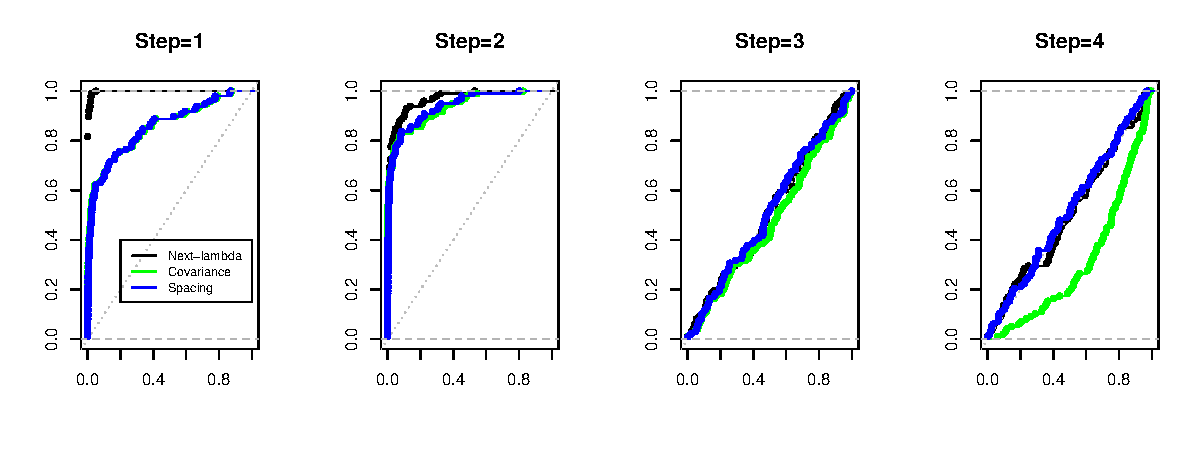
\includegraphics[width=\textwidth]{figs/larexample.pdf}
  \caption[fig:larexample]{\em  Cumulative distribution functions of p-values for LAR/lasso tests from simulations with $N=50,  p=10$ and two strong signals.}
  \label{fig:larexample}
\end{figure}

\subsection{Comparison of Selected- and Saturated-Model Inference}\label{sec:bivariate}


Selected-model inference is typically more computationally involved than saturated-model inference. Because the saturated-model test conditions on $n-1$ dimensions, the resulting distribution in~\eqref{eq:satModel} is nothing more than a truncated univariate Gaussian random variable. By contrast, selected-model tests typically require sampling from a truncated multivariate Gaussian distribution of dimension $p-|E_{k-1}|$.

For some applications, a major conceptual advantage of the saturated-model approach is that, when $M(E)$ is misspecified, $\theta^{E}$ is still a well-defined quantity on which we can perform exact inference. For example, a 95\% confidence interval for $\theta_{j_k}^{E_k}$ could cover that coefficient with probability 95\% even if $M(E_k)$ is misspecified. In the setting of sequential model selection, this advantage is less important. We do not necessarily need a scientifically interpretable interval for $\theta_{j_k}^{E_k}$; rather, the goal of the test at step $k$ is to reject $M_{k-1}$ and move on if it is demonstrably incompatible with the data.

There are several major benefits to selected-model inference. First, selected-model inference allows us to drop the assumption that $\sigma^2$ is known by conditioning on $\|Y\|^2$, the sufficient statistic corresponding to the natural parameter $1/2\sigma^2$. This is not an option for the saturated model because conditioning on both $\|Y\|^2$ and $\proj_{\eta_k}^\perp Y$ results in a degenerate conditional distribution for $\eta_k'Y$.  See \citet[][Section 5]{fithian2014optimal} for a detailed discussion of the distinctions between saturated-model and selected-model tests.

Second, we have seen in Section~\ref{sec:pValsIndep} that tests of the form~\eqref{eq:selModel_cond} or~\eqref{eq:selModel_marg} yield independent $p$-values under general conditions, allowing us to apply  the sequential stopping rules of~\citet{gsell2013sequential} and \citet{li2015accumulation}.

Finally, and perhaps most importantly, selected-model tests can be dramatically more powerful than saturated-model tests, as we illustrate now with an extended example.

\begin{example}[Bivariate Regression with Identity Design]\label{ex:bivariate}
  Consider forward stepwise selection in a regression model with $n=p=2$, with known $\sigma^2=1$ and identity design 
\[
X = I_2=\begin{pmatrix} 1 & 0 \\ 0 & 1\end{pmatrix}.
\] 

The forward stepwise path and the lasso path both select $j_1=1$ if and only if $|Y_1|>|Y_2|$. The selection event $A_1=\{|Y_1| > |Y_2|\}$ is shown in yellow in Figure~\ref{fig:bv_condSets}. If $j_1=1$ then
\[
M_0:\; Y\sim \cN(0,I_2), \quad\text{ and } 
M_1:\; Y \sim \cN\left(\binom{\mu_1}{0}, \; I_2\right).
\]

The selected-model test at step 1 compares $Y_1$ to its distribution under $M_0$ conditional on $A_1$, a test of $H_0:\;\mu_1=0$ in model $M_1$. By contrast, the saturated-model test is a test of $H_0:\; \mu_1=0$ in the model $M_{\text{sat}}:\; Y \sim \cN(\mu, I_2)$. The saturated model test must condition on $Y_2$ to eliminate the nuisance parameter $\mu_2$, and compare $Y_1$ to its null distribution given $A_1$ {\em and} the observed value of $Y_2$.

Figure~\ref{fig:bv_condSets} shows the conditioning sets for each model when $Y=(2.9, 2.5)$. Next to it, Figure~\ref{fig:bv_nullDists} shows the null distribution for the test statistic $Y_1$ in each case. The $p$-values for the selected and saturated models are 0.007 and 0.3, respectively. These two plots are reproduced from \citet{fithian2014optimal}, in which the same example was presented in less detail.
\end{example}

\begin{figure}
  \centering
  \begin{subfigure}[t]{.4\textwidth}
    % source code: bivariateSelVSat.R
    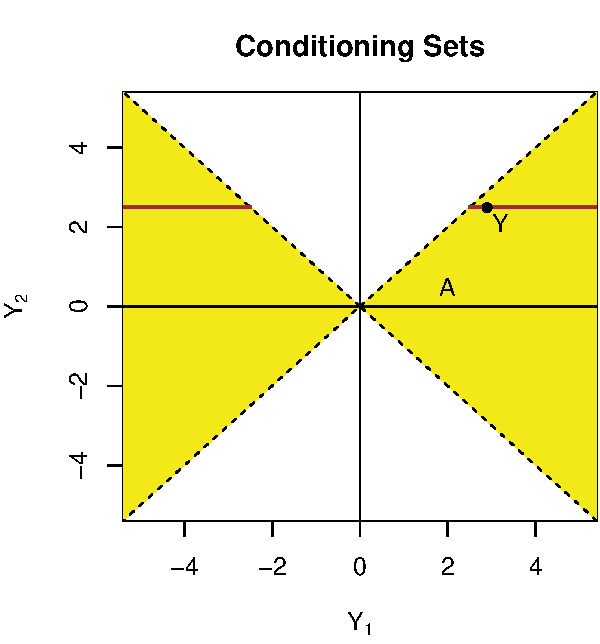
\includegraphics[width=\textwidth]{figs/bivariateSelVSat_condSets.pdf}
    \caption{The selected-model test conditions on $j_1=1$ (yellow region), while the saturated-model test also conditions on $Y_2=2.5$ to eliminate the nuisance variable $\mu_2$ (brown region).}
    \label{fig:bv_condSets}
  \end{subfigure}
  \hspace{.1\textwidth}
  \begin{subfigure}[t]{.4\textwidth}
    % source code: bivariateSelVSat.R
    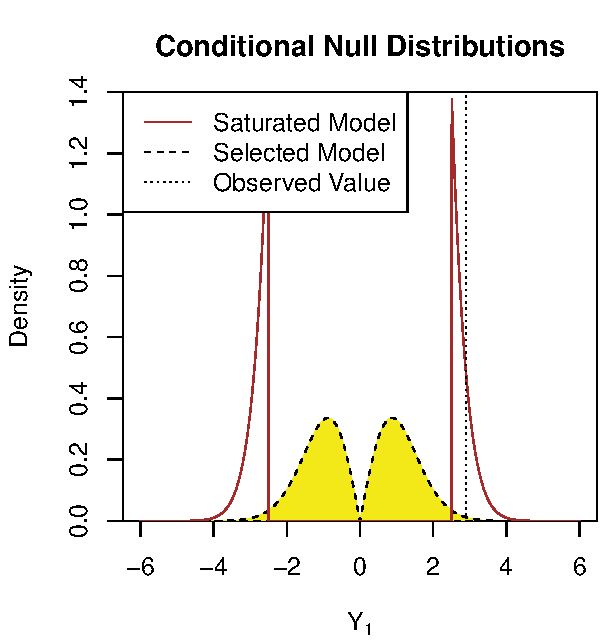
\includegraphics[width=\textwidth]{figs/bivariateSelVSat_nullDists.pdf}
    \caption{Conditional distributions of $Y_1$ under
      $M_0:\; Y \sim \cN(0,I_2)$. The realized value $|Y_1|=2.9$ is
      quite large given that $j_1=1$. By
      contrast, $|Y_1|=2.9$ is not especially large once we 
      also condition on $Y_2=2.5$.}
  \end{subfigure}
  \caption{Contrast between the saturated-model and selected-model
    tests in Example~\ref{ex:bivariate}. The selected-model test is based on  $\L(Y_1 \gv j_1=1)$,  whereas the saturated-model test is based on $\L(Y_1  \gv Y_2, \; j_1=1)$. 
    When $Y=(2.9, 2.5)$, the selected- and saturated-model $p$-values are 0.015 and 0.3, respectively.}
  \label{fig:bv_nullDists}
\end{figure}


Figure~\ref{fig:bv_condSets} illustrates a certain phenomenon occurring in saturated-model tests: when there are near-ties between strong variables that are competing to enter the model, the resulting $p$-value my be very weak~\citep{lockhart2014significance}. Figure~\ref{fig:bv_rocCurve} displays the cumulative distribution function for the first $p$-value when $\mu=(4,4)$, a very strong signal. While the selected model test has near perfect power, it is not uncommon for the saturated model test to produce large $p$-values, even in the range of 0.5-0.9. These large $p$-values arise when there is a near tie between the variables.

\begin{figure}
  \centering
  % source code: bivariateSelVSat.R
  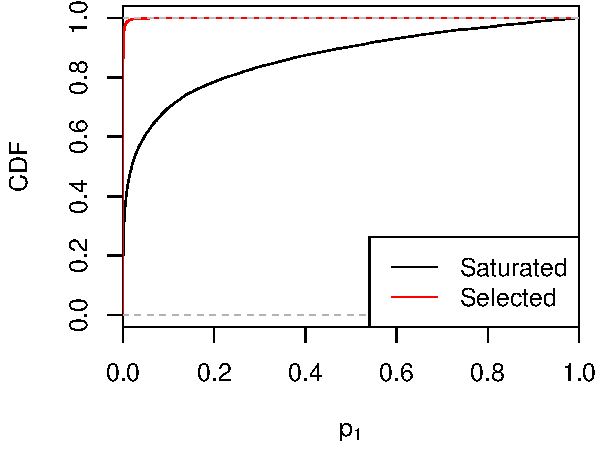
\includegraphics[width=.5\textwidth]{figs/bivariateSelVSat_rocCurve.pdf}
  \caption{Cumulative distribution function of $p_1(Y)$ for the selected- and saturated-model tests when $\mu=(4,4)$. Even though the signal is very strong, the saturated-model test results in large $p$-values in realizations like the one in Figure~\ref{fig:bv_nullDists}, where there is a near-tie between $|Y_1|$ and $|Y_2|$. By contrast, the selected-model test has nearly perfect power.}
  \label{fig:bv_rocCurve}
\end{figure}

Results in \citet{fithian2014optimal} show that the selected-model test is strictly more powerful when the selected model is correct; i.e., when $\mu_2=0$. Figure~\ref{fig:bv_powCurves} shows the power curve for each test when $\mu_2=0$ (left panel) and $\mu_2=4$ (right panel). While the selected-model test is more powerful when the selected model is correct, the difference between the two is relatively small. The difference is much more pronounced when $\mu_2=4$. 

Note that if $\mu=(0,4)$, the incremental null is true, but the complete null is false. That is, the model $M_0 = M(\emptyset)$ is missing an important signal variable, but the missing variable is not $X_1 = (1,0)$. Because the saturated-model test is really a test of the incremental null, its power is $\alpha=0.05$. By contrast, the selected-model test rejects about half the time when $\mu=(0,4)$, successfully detecting the fact that $M_0$ is a poor fit to the data.

\begin{figure}
  \centering
  \begin{subfigure}[t]{.4\textwidth}
    % source code: bivariateSelVSat.R
    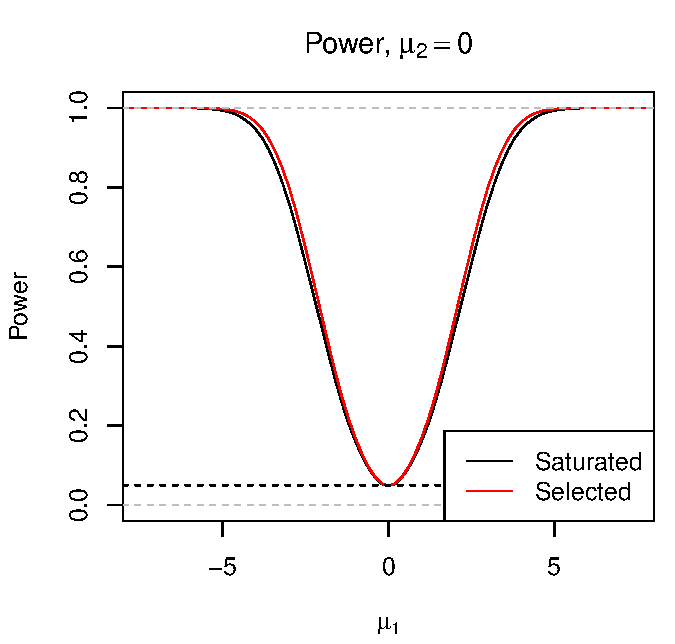
\includegraphics[width=\textwidth]{figs/bivariateSelVSat_powCurves_0.pdf}
    %\caption{\WFcomment{Write caption here.}}
    %\label{fig:bv_powCurves_0}
  \end{subfigure}
  \hspace{.1\textwidth}
  \begin{subfigure}[t]{.4\textwidth}
    % source code: bivariateSelVSat.R
    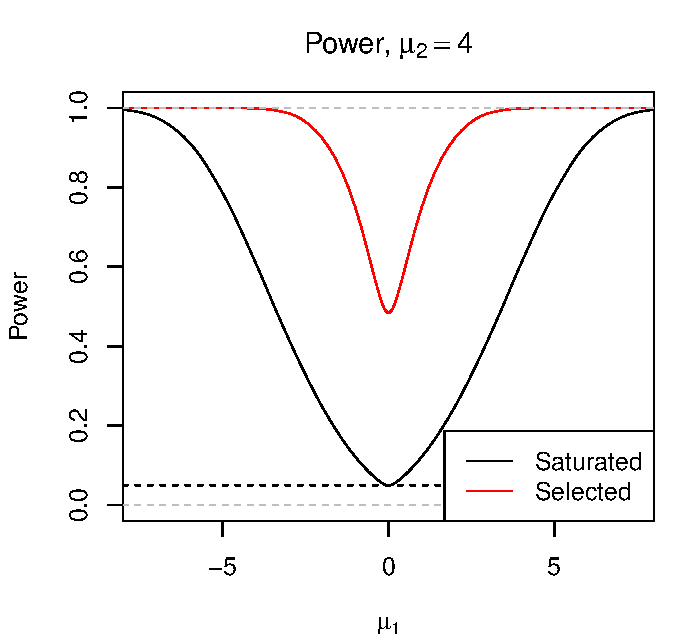
\includegraphics[width=\textwidth]{figs/bivariateSelVSat_powCurves_4.pdf}
    %\caption{\WFcomment{Write caption here.}}
  \end{subfigure}
  \caption{Power at level $\alpha=0.05$ for saturated- and selected-model tests at step 1, given that $j_1=1$. The power is plotted as a function of $\mu_1$, for two different values of $\mu_2$. When $\mu_2=0$, the selected-model test is strictly more powerful than the saturated-model test, but the difference is slight. By contrast, when $\mu_2=4$, the selected-model test is much more powerful. The dashed line shows $\alpha=0.05$.}
   \label{fig:bv_powCurves}
\end{figure}

Saturated-model $p$-values are generically non-independent. Continuing with Example~\ref{ex:bivariate}, Table~\ref{tab:bv_twoWayTable} shows a two-way contingency table for the saturated-model $p$-values $(p_1(Y), p_2(Y))$, binned into cells of height and width 0.2, simulated under the global null $\mu=0$. Because $k_0=0$, both $p$-values are uniform by construction, but the $p$-values are strongly dependent, with correlation $-48\%$. By contrast, the selected-model $p$-values $(p_1,p_2)$ are independent under the global null, a consequence of Theorem~\ref{thm:suffCond}.

\begin{comment}
Computing the cutoff for the saturated-model test requires us to know $\proj_{\eta}^\perp Y$, which is not $\sF_k$-measurable.

By contrast, selected-model tests of $M_{k-1}$ against $M_k$ are always $\sF_k$-measurable, because they are based on the law
\begin{equation}\label{eq:selModel}
\L\left(X_{j_k}'Y \mid X_{E_k-1}'Y, E_{k-1}, j_k\right),
\end{equation}
and all of the random variables appearing in~\eqref{eq:selModel} are $\sF_k$-measurable.
\end{comment}

% latex table generated in R 3.0.2 by xtable 1.7-1 package
% Mon May  4 21:11:15 2015
\begin{table}[ht]
  \centering
  \begin{tabular}{l|ccccc|c}
    \multicolumn{7}{c}{Saturated-Model $p$-Values 
      (\% of $10^6$ Simulations)}\\[7pt]
    \hline
    \multicolumn{7}{c}{}\\[-1.5ex]
    \multicolumn{7}{c}{$p_2(Y)$}\\[5pt]
    ${\large p_1(Y)}$ & (0,0.2] & (0.2,0.4] & (0.4,0.6] & (0.6,0.8] & (0.8,1] & \textbf{Total} \\ 
    \hline
    (0,0.2] & 1.0 & 2.7 & 4.2 & 5.6 & 6.7 & 20.1 \\ 
    (0.2,0.4] & 1.4 & 3.4 & 4.5 & 5.2 & 5.5 & 20.0 \\ 
    (0.4,0.6] & 2.3 & 4.3 & 4.7 & 4.5 & 4.2 & 20.0 \\ 
    (0.6,0.8] & 4.2 & 5.4 & 4.3 & 3.4 & 2.7 & 20.0 \\ 
    (0.8,1] & 11.1 & 4.3 & 2.3 & 1.4 & 1.0 & 20.0 \\ 
    \hline
    \textbf{Total} & 19.9 & 20.0 & 20.0 & 20.1 & 20.0 & 100.0 \\ 
    \hline
  \end{tabular}
  \caption{Two-way contingency table of saturated-model $p$-values $(p_1(Y), p_2(Y))$ for Example~\ref{ex:bivariate}, after binning into cells of height and width 0.2. We report the percentage of $p$-value pairs falling into each cell out of one million simulations from the global null hypothesis, $\mu=0$. Both $p$-values are marginally uniform but strongly dependent, with a correlation of $-48\%$.}
\label{tab:bv_twoWayTable}
\end{table}

\begin{comment}
First, note that $p_2$ is a selective $p$-value for comparing the null with only variable 1,
\[
M_1:\; Y \sim \cN\left(\binom{\mu_1}{0}, I_2\right),
\]
against the alternative with variables 1 and 2:
\[
M_2:\; Y \sim \cN\left(\mu, I_2\right), \text{ with } 
\mu_2 \neq 0.
\]
To eliminate the nuisance parameter $\mu_1$, the test conditions on $Y_1$. Thus, $p_2$ is uniform given $Y_1$ on $A$. Second, note that on $A$, $p_1$ is a function only of $Y_1$. Thus, $(p_1,p_2)$ are independent uniform variables given that variable 1 is chosen first. By a similar argument, they would also be independent uniforms if $Y_2$ were chosen first; thus, $(p_1, p_2)$ are marginally uniform under the global null.
\end{comment}

\section{Computation}
\label{sec:computation}

As usual, we have reduced computation of the $p$-value at step $k$ to a sampling problem. Whatever our test statistic at step $k$, we must compute its distribution under the null model $M_{k-1}$. We give details of our  strategy here for the max-t test in forward stepwise regression.


Given a model $M_{k-1}$   we need to sample from 
\begin{eqnarray}
L(X'_jY | E_{k-1},X'_{E_{k-1}})
\label{eqn:maxtsamp}
\end{eqnarray}
with $Y\sim N(\mu, I \cdot \sigma^2)$.
The current model fit is $\proj_{E_{k-1}} Y$ and it is easy to see that (\ref{eqn:maxtsamp})  is equivalent to sampling
\begin{eqnarray}
Y^*=\proj_{E_{k-1}} Y + (I- \proj_{E_{k-1}}) Z; \;Z\sim N(0,I\cdot\sigma^2)
\label{eq:boot}
\end{eqnarray}
and then conditioning on the event $E_{k-1}(Y^*)= E_k(Y)$ (a polyhedron).
In other words, we need to condition on data vectors  $Y*$ that yields the same
sequence of variables and coefficient signs up to step $k-1$. This is the challenging aspect of this computation.

Note that  (\ref{eq:boot})  has the form of  (conditional) parametric bootstrap sampling, in which the bootstrap residuals projected into the subspace
orthogonal to the current fit. In similar fashion, one might use a instead a nonparametric version of (\re{eq:boot}), sampling
with replacement from the model residuals and then projecting them orthogonal to the current model.

Figure \ref{fig:comparison} shows and example with $n=100,p=20$ and one strong signal, computing the max-t pvalue at Step 3.
The ``exact'' answer  was determined from bootstrap sampling with $20,000$ replications.
The Figures show the bias, variance and MSE of the estimates from accept/reject and hit and run, using between 1000 and 8000 samples, averaged
over 10 different starting seeds.
\begin{figure}[htp]
\centering
  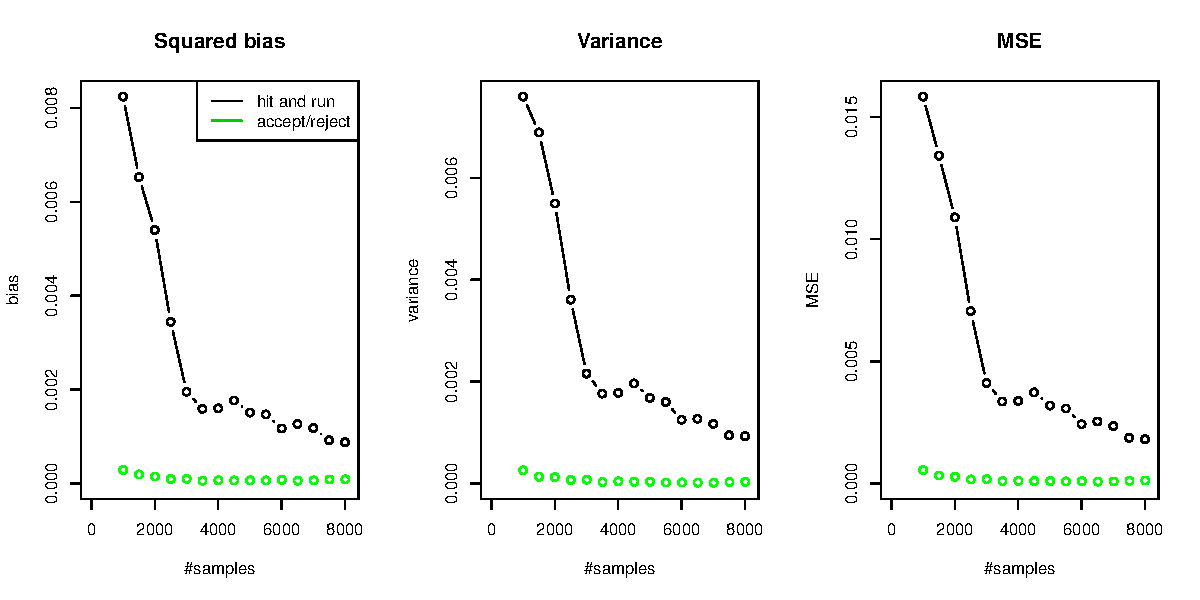
\includegraphics[width=\textwidth]{figs/comparison.pdf}
  \caption{\em Simulated example with $n= 100, p=20$ and one strong signal, computing the max-t pvalue at Step 3.  Shown are bias, variance and MSE of the estimates from accept/reject and hit and run, using between 1000 and 8000 samples, averaged
over 10 different starting seeds.
}
  \label{fig:comparison}
\end{figure}
We see that accept/reject is far more efficient, yielding a smaller MSE with 1000 samples then hit and run gives for  8000 samples.
Hence we use accept/reject for as many steps of the sequence is possible,  until the point where the acceptance rate is too low to make is practical.

In detail, we employ a hybrid computational strategy; we use accept-reject sampling, and do so as long as we obtain at least 300 (say) samples in the first set
of $B$ realizations ($75,000$ in our code)  This is an effective approach until we have reached a point in the model path where all predictors have little or no signal.
When the acceptance rate gets too low, we switch to a hit-and run Monte Carlo approach. We exploit the fact that each move along a random direction 
has a truncated Gaussian distribution whose truncation limits are easily computed from the properties of the polyhedral. Unlike accept-reject, sampling
which produces independent samples,  the hit and run method produces dependent samples. Hence we must run it for longer with an initial burn in period,
and hope that it has mixed sufficiently well.



The task is made much simpler by the fact that the selection event can we written as $S_M=\{y: \Gamma y \geq u\}$.
Hence we don't need to run the entire forward stepwise procedure on $y^*$: instead, we pre-compute $\Gamma$ and $u$ and then check
if $\Gamma y^* \geq u$. Further, since $\Gamma$ has on the  order of $2pk$ rows after $k$ steps,  we can save 
substantially in computation by checking the row-wise inequalities starting from the last row, where the inequality is most likely to fail.

\subsection{Reducing the number of constraints}
Happily, it turns out that the conditioning polytope can be expressed with only $2p$ constraints in forward stepwise regression, as we show here.
This increases the speed of both accept/reject and hit and Run sampling for our problem.

\begin{theorem}
  Assume the model path $M_{0:d}$ is obtained by forward stepwise 
  linear regression. Then, for a candidate active set $E$ of size $k$, 
  the set $A = \{E_k = E, \;X_E'Y = u\}$ is characterized 
  exactly by the constraints $X_E'Y=u$ and
  \[
  v_j^-(E,u) < X_j'Y < v_j^+(E,u), \quad\forall j \notin E,
  \]
  for $v_j^-$ and $v_j^+$ given explicitly in
  Equations~(\ref{eq:vMinus_FS}--\ref{eq:vPlus_FS}).
  Thus, $A$ corresponds exactly to 
  a set with $2(p-k)$ linear inequality constraints and $k$
  linear equality constraints on $Y$.
\end{theorem}

\begin{proof}
  At stage $i < k$, the next variable to enter is the one with maximal correlation with the residual vector; i.e.
  \[
  j_{i+1} = \argmax_{j \notin E_i} 
  \frac{\left| X_j ' (Y - X_{E_i}\hat\beta^i) \right|}
  {\|\proj_{E_i}^\perp X_j\|}
  \]
  The crucial observation is that, 
  once we know the $k$th active set 
  $E_k$ and its sufficient statistics
  $X_{E_k}'Y$, we know the entire 
  path of fitted models up to step $k$.
  On the set $\{E_k=E\}$, all of the quantities 
  $j_{i+1}$, $E_i$, $\hat\beta^i$, and $\proj_{E_i}^\perp$
  depend only on $X_E'Y$. For brevity, write
  \[
  C_i^* = \max_{j \notin E_i} 
  \frac{\left| X_j ' (Y - X_{E_i}\hat\beta^i) \right|}
  {\|\proj_{E_i}^\perp X_j\|}.
  \]
  On $A$, $C_i^*$ is attained at $j=j_{i+1}$, the $i$th 
  variable added.

  If $X_E'Y$ is fixed at $u$, and $j \notin E$, then the condition for 
  $X_j$ {\em not} to enter at step $i+1 < k$ is
  \[
  \frac{\left| X_j' (Y - X_{E_i}\hat\beta^i) \right|}
  {\|\proj_{E_i}^\perp X_j\|} 
  \leq C_i^*,
  \]
  or equivalently,
  \begin{equation}\label{eq:noEnterBounds_FS}
    X_j' X_{E_i}\hat\beta^i -
    C_i^*\|\proj_{E_{i}}^\perp X_{j}\|
    \;\;\;\leq\;\;\;
    X_j'Y
    \;\;\;\leq\;\;\;
    X_j' X_{E_i}\hat\beta^i +
    C_i^*\|\proj_{E_{i}}^\perp X_{j}\|, 
  \end{equation}
  so the set $A$ is equivalent to 
  Equation~\eqref{eq:noEnterBounds_FS} holding
  for every $i < k$ and $j \notin E$. Nominally, this gives $2k(p-k)$
  linear inequality constraints to satisfy, but most of them are
  non-binding. On $A$, the upper and lower bounds
  in~\eqref{eq:noEnterBounds_FS}
  are all known functions of $E$ and $u$, so we can set
  \begin{align}\label{eq:vMinus_FS}
    v_j^-(E,u) &= \max_{0 \leq i < k} \;\;X_j' X_{E_i}\hat\beta^i -
    C_i^*\|\proj_{E_{i}}^\perp X_{j}\| \\
    \label{eq:vPlus_FS}
    v_j^+(E,u) &= \min_{0 \leq i < k} \;\;X_j' X_{E_i}\hat\beta^i +
    C_i^*\|\proj_{E_{i}}^\perp X_{j}\|.
  \end{align}  
\end{proof}

As we see below, a similar result holds for the LASSO ever-active path. In fact, it holds for a much larger class of $\ell_1$-regularized exponential family models including the graphical LASSO.

\begin{theorem}
  Assume that $M_\infty$ is an exponential family model
  of the form
  \[
  Y \sim \exp\{ \theta'U(y) - \psi(\theta) \}\,d\nu(y),
  \]
  with $\Theta \sub \R^p$ convex, and assume
  that the model path $M_{0:d}$ is given 
  by the ever-active set for the $\ell_1$-penalized problem
  \begin{equation}\label{eq:regProblem}
  \hat\theta^r = \argmin_{\theta\in \Theta} 
  -\ell(\theta) + \lambda_r\|\theta\|_1,
  \end{equation}
  for some sequence $\lambda_r > 0$.

  Then, for a candidate active set $E$ of size $k$, 
  the set $A = \{E_k = E, \;U_E = u\}$ is characterized 
  exactly by the constraints $U_E = u$ and
  \[
  v_j^-(E,t) \leq U_j(Y) \leq v_j^+(E,t), \quad\forall j \notin E,
  \]
  for $v_j^-$ and $v_j^+$ given explicitly in
  Equations~(\ref{eq:vMinus_L1}--\ref{eq:vPlus_L1}).
  Thus, $A$ corresponds exactly to 
  a set with $2(p-k)$ linear inequality constraints and $k$
  linear equality constraints on $U(Y)$.
\end{theorem}

\begin{proof}
  Note that, because exponential family likelihoods are concave in their natural parameters, the problem in~\eqref{eq:regProblem} is convex. Again, once we know the sufficient statistics $U_E(Y)$ for model $k$, and that $E_k=E$, we know that
  \[
  \hat\theta^r = \hat\theta^{(E,r)}
  \]
  for every $r \leq R_k$, so we know the entire path of fits up to and including $R_k$. But then, excluding variable $j \notin E$ at Lagrange parameter $\lambda_r$ is equivalent to
  \[
  \lambda_r \geq 
  \left| \pardd{\ell(\hat\theta^r)}{\theta_j} \right|
  = \left|U_j - \E_{\hat\theta^r}[U_j]\right|
  \]
  On $A$, for $r \leq R_k$, 
  $\E_{\hat\theta^r}[U_j]$ is a known function of $E$ and $u$,
  so we can set
  \begin{align}\label{eq:vMinus_L1}
    v_j^-(E,u) &= \sup_{r \leq R_k} \;\; 
    \E_{\hat\theta^r}[U_j] - \lambda_r \\
    \label{eq:vPlus_L1}
    v_j^+(E,u) &= \inf_{r \leq R_k} \;\;
    \E_{\hat\theta^r}[U_j] + \lambda_r .
  \end{align}
\end{proof}

\WFcomment{Give more general characterization of when we can do it, including group lasso? QP? Generalized Lasso?}

\begin{comment}
\subsection{An analytic approximation for the max-t test}
 Suppose we have taken $k$ steps of forward stepwise regression with $p$ predictors and let the selected model  
 be $E$. Suppose we choose predictor $j^*$ at the next step.
 
Let $T_j=\eta_j^Ty, j \notin M$ be the partial regression coefficients for all predictors not in $E$,
and $(v_j^-, v_j^+)$ be the limits derived from the polyhedral lemma applied to $(E, \eta_j)$  (See e.g. \citet{spacings}).
These are the upper and lower bounds for the functional $\eta_j^Ty$ implied by the event that model $E$ is selected from the data $y$.
We chose the sign of $\eta_j$ so that $\eta_j^Ty$ is  $\geq 0$. 

 Let $F_{\mu,\sigma^2}^{a,b}(t)$ be the  cumulative distribution function of the truncated normal.
 Finally let $T=|T_{j^*}|$.
Then by assuming independence, a  simple approximation to the max-t value is given by
\begin{equation}
1-\prod_{j\notin E} \{F_{0,||\eta||^2}^{v_j^-, v_j^+}(T)-   F_{0,||\eta||^2}^{v_j^-, v_j^+}(-T) \}
\label{eqn:approxpv}
\end{equation}
This approximation is exact if the predictors are uncorrelated.

Figure \ref{fig:approxpv} shows an example with $n=50$ and $p=10$ features having pairwise correlation 0.5.
There are two moderate signals.
Shown are the p-values from the ``exact'' numerical computation (with $100,000$ bootstrap samples)
and the approximation based on (\ref{eqn:approxpv}).
\begin{figure}[htp]
\centering
  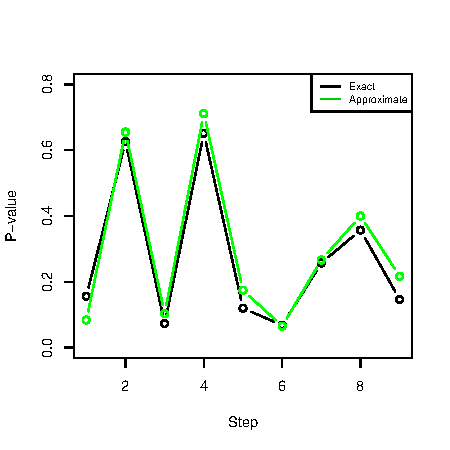
\includegraphics[width=3in]{figs/approxpv.pdf}
  \caption{Exact max-t pvalues and approximation based on (\ref{eqn:approxpv}), for a simulated example
  with $n=50, p=10$.}
  \label{fig:approxpv}
\end{figure}
The approximation seems quite good. By Sidak's lemma, we might conjecture that the approximation is conservative, but we have no proof of this.
\end{comment}

\section{Simulation: Sparse Linear Regression}
\label{sec:sparseReg}

Next we compare several model selection procedures in simulation. We simulate from a linear regression model with $n=100$ observations and $p=40$ variables. The design matrix $X\in\R^{n\times p}$ is a random Gaussian design with pairwise correlations of 0.3 between predictor variables.

The columns of $X$ are normalized to have length 1, and we simulate from $Y \sim \cN(X\beta,I_n)$, using a seven-sparse model with signal-to-noise ratio 5:
\[
\beta_j = \left\{\begin{matrix}5 & j = 1,\ldots,7\\ 0 &
    j>7\end{matrix}\right.
\]
We use known $\sigma^2=1$, so that we can compare the saturated-model test with the selected-model test. For our selection algorithm, we use the entire forward-stepwise path, for all 40 steps. 

\subsection{Single-Step $p$-Values}

For each step we compute one-step selected-model and saturated-model $p$-values, as well as nominal (unadjusted) $p$-values, conditioning on the signs of the active variables to make the problem more computationally tractable. Figure~\ref{fig:simulation_null_false} shows the power of all three tests for each of the first ten steps, conditional on the event that the null hypothesis is false. It is clear from Figure~\ref{fig:simulation_null_false} that the selected-model $p$-values are far more powerful than the saturated-model $p$-values. The nominal $p$-values are also quite powerful, but they do not have the correct level.

\begin{figure}[h]
  \centering
  % source code: ??? for simulation, sparseSim.R for plotting
  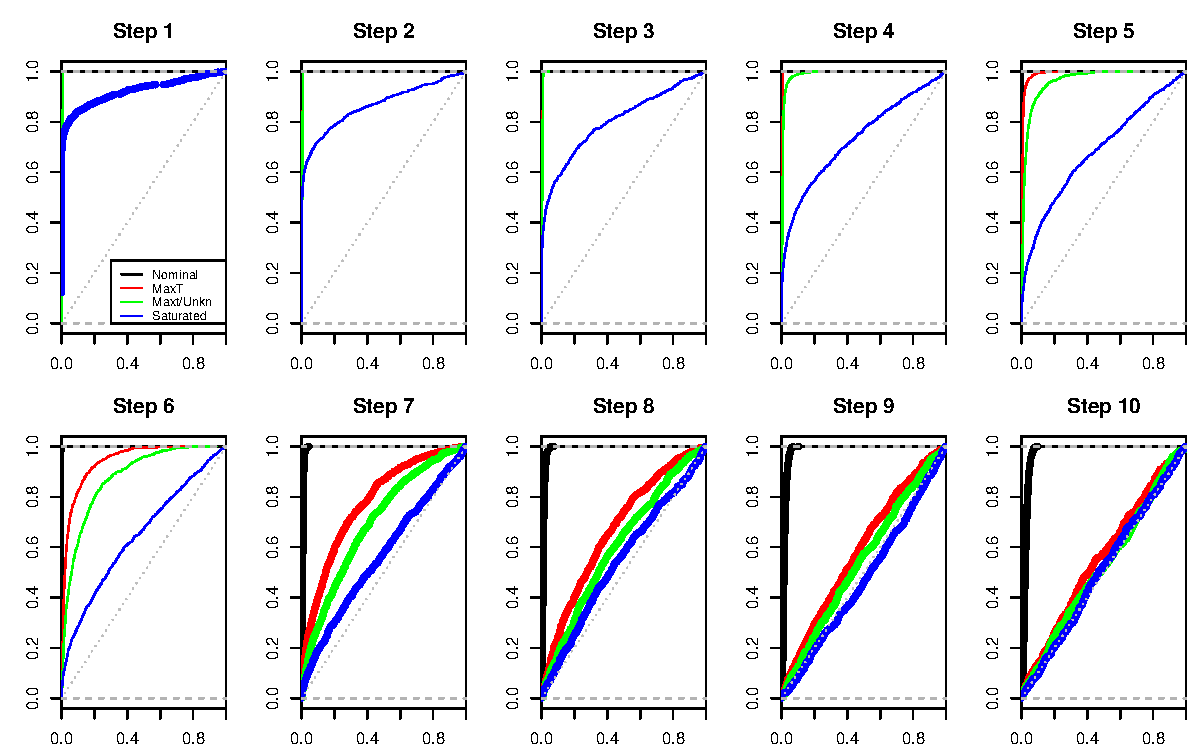
\includegraphics[width=1\textwidth]{figs/simulation_snr_5_alpha_05_null_false.pdf}
  \caption{\em  CDFs of nominal (black), MaxT (red), MaxT with unknown $\sigma$ (green) and  saturated-model (blue) $p$-values in the simulation of Section~\ref{sec:sparseReg}, conditional on testing a false null hypothesis at step $k$. The MaxT approaches are much more powerful than the saturated-model test. The nominal test appears to be powerful, 
  but is not $U(0,1)$ under the null, as shown below in Figure \ref{fig:simulation_null_true}.}
  \label{fig:simulation_null_false}
\end{figure}

\begin{figure}[h]
  \centering
  % source code: ??? for simulation, sparseSim.R for plotting
  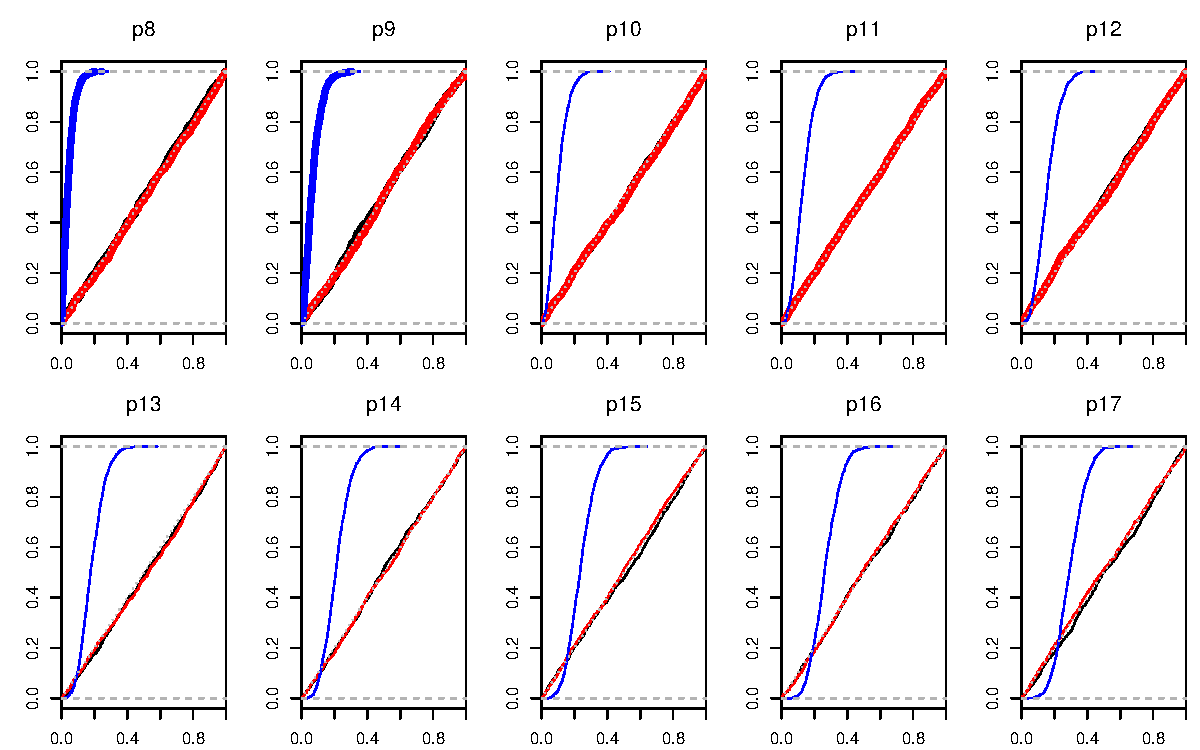
\includegraphics[width=1\textwidth]{figs/simulation_snr_5_alpha_05_null_true.pdf}
  \caption{\em  CDFs of nominal (black), MaxT (red), MaxT with unknown $\sigma$ (green) and  saturated-model (blue) p-values in the simulation of Section~\ref{sec:sparseReg}, conditional on testing a true null hypothesis at step $k$.  The nominal test is badly anti-conservative, while all of the other methods  show uniform p-values as desired.}
  \label{fig:simulation_null_true}
\end{figure}

\begin{figure}[h]
  \centering
  % source code: ??? for simulation, sparseSim.R for plotting
  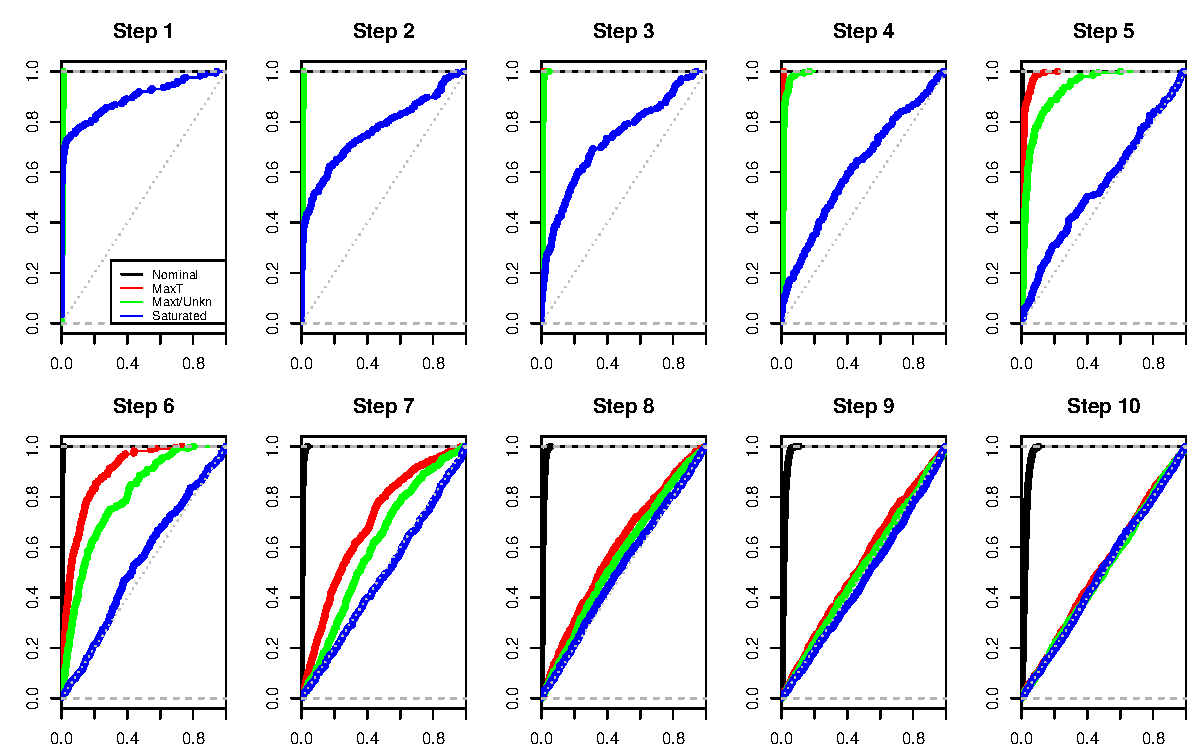
\includegraphics[width=1\textwidth]{figs/simulation_snr_5_alpha_05_noise_var.pdf}
  \caption{\em CDFs of nominal (black), MaxT (red), MaxT with unknown $\sigma$ (green) and  saturated-model (blue) $p$-values in the simulation of Section~\ref{sec:sparseReg}, conditional on the event that the variable added at step $k$ is a noise variable in the full model. Here, none of the methods produce uniform $p$-values. The null hypothesis is false in most cases and so --- in our model-centric point of view --- rejection is the desired outcome.}
  \label{fig:simulation_noise_var}
\end{figure}

Figure~\ref{fig:simulation_null_true} shows the distribution of $p_k$ for $k = 8, \ldots, 17$, given that the null hypothesis tested at step $k$ is correct (i.e., that $k_0< k$). Because the correct model is seven-sparse, $k=8$ is the first index for which the null can possibly be true. Both selective $p$-values are uniform by construction, but the nominal $p$-values are highly anti-conservative, as expected.

Finally, as a warning against misinterpretation of our method, we include Figure~\ref{fig:simulation_noise_var} showing the first ten $p$-values for each method, conditional on event that the variable added at step $k$ is a noise variable in the full model. Now, none of the $p$-values are uniform. 

This is {\em not} a mistake in our implementation of the method, but rather a consequence of our ``model-centric'' point of view. If we try to add a noise variable to the model before we have included all the signal variables, then we are testing a false null hypothesis. The test rejects because there is much more signal to find, and as such, it is entirely appropriate for us to reject the null and continue growing the model.

\subsection{Model-Selection Performance}

If we combine the saturated-model or selected-model $p$-values with one of our three stopping rules, we can evaluate the model-selection performance of each method in terms of:
\begin{itemize}
\item its probability of selecting a correct model or $p_{\text{screen}}$,
\item its model-wise FWER,
\item its model-wise FDR, and
\item its variable-wise FDR, where we use $\tV= \#\{\text{ noise variables included in } M_{\hk}\}$ instead of $V=(\hk-k_0)_+$.
\end{itemize} 
The last measure of performance is not explicitly controlled by any of the selective-inference methods, but we might nevertheless hope to perform reasonably. \WFcomment{Comment on results once they are correct. These numbers are wrong right now.}

\WFcomment{Should we compute the FWER and FDR only conditional on screening? Strong / Forward / Basic should all be correct given screening since they condition on $p_{1:k_0-1}$.}

% latex table generated in R 3.0.2 by xtable 1.7-1 package
% Fri May  1 09:29:28 2015
%\begin{table}[ht]
 % \centering
 % \begin{tabular}{llcccc}
  %  \hline
  %  Method & Stopping Rule & $p_{\text{screen}}$ & $\text{FWER}_{\text{mod}}$ an
 %   & $\text{FDR}_{\text{mod}}$ 
  %  & $\text{FDR}_{\text{var}}$ \\ 
 %   \hline
    %Selected & Basic & .290 & .000 & .002 & .039 \\ 
   % Selected & Forward & .559 & .027 & .020 & .066 \\ 
   % Selected & Strong & .041 & .014 & .008 & .042 \\ 
  %  \hline
   % Saturated & Basic & .000 & .000 & .000 & .028 \\ 
  %  Saturated & Forward & .014 & .000 & .000 & .030 \\ 
  %  Saturated & Strong & .000 & .000 & .000 & .032 \\ 
  %  \hline
  %  Knockoffs & & .000 & --- & --- & .231 \\ 
  %  \hline
 % \end{tabular}
 % \caption{\WFcomment{Comment on results once they are correct. These numbers are wrong right now.}}
%\end{table}

\begin{table}[ht]
\centering
\begin{tabular}{rrrrr}
  \hline
  Method, Stopping rule& $p_{\text screen}$ & FWER$_{\text mod}$ & FDR$_{\text mod}$ &FDR$_{\text var}$ \\
% & \$p\_\{$\backslash$text\{screen\}\} & \$$\backslash$text\{FWER\}\_\{$\backslash$text\{model\}\}\$ & \$$\backslash$text\{FDR\}\_\{$\backslash$text\{model\}\}\$ & \$$\backslash$text\{FDR\}\_\{$\backslash$text\{variable\}\}\$ \\ 
  \hline
Nominal, Simple & 0.832 & 0.252 & 0.097 & 0.171 \\ 
  Nominal, Forward & 0.931 & 0.896 & 0.345 & 0.426 \\ 
  Nominal, Strong & 0.003 & 0.000 & 0.000 & 0.035 \\ 
  \hline
  MaxT, Simple & 0.369 & 0.000 & 0.002 & 0.042 \\ 
  MaxT, Forward & 0.668 & 0.038 & 0.026 & 0.080 \\ 
  MaxT, Strong & 0.025 & 0.006 & 0.004 & 0.038 \\ 
  \hline
  MaxT-Identify, Simple & 0.404 & 0.000 & 0.002 & 0.042 \\ 
  MaxT-Identify, Forward & 0.688 & 0.039 & 0.026 & 0.082 \\ 
  MaxT-Identify, Strong & 0.024 & 0.003 & 0.002 & 0.037 \\ 
  \hline
  Saturated, Simple & 0.000 & 0.000 & 0.000 & 0.029 \\ 
  Saturated, Forward & 0.013 & 0.001 & 0.000 & 0.030 \\ 
  Saturated, Strong & 0.000 & 0.000 & 0.000 & 0.033 \\ 
  \hline
  Knockoffs & 0.252 &  &  & 0.103 \\ 
   \hline
\end{tabular}
\caption[tab:stopping]{\em Results of various stopping rules applied to simulated data with 7 strong signals,  as described at the beginning of Section \ref{sec:sparseReg}.
The {\tt Simple} rule stops at the first time that a p-value exceeds $\alpha$, while {\tt Forward} and {\tt Strong} refers to the ForwardStop and StrongStrop rules of Section \ref{sec:sequential}.}
\label{tab:stopping}
\end{table}

We see that 1) strongStop and forwardStop control FWER and modelwise FDR, respectively, using p-values from MaxT or MaxT-identify, as predicted by theory
2) the nominal p-values do not lead to control of FWER or FDR, as expected, 3) the pvalues from the saturated model show FWER and modelwise-FDR control,
although not guaranteed by theory, 4) the MaxT rules show higher probabilities of selecting the true model, especially using forwardStop, 5) the knockoff method
does not yields variable-wise FDR control, as it should.
5)
\section{Principal Components Analysis}
\label{sec:pca}

\WFcomment{Can we do this one?}
Here we consider model selection for   principal components analysis. In that case we are given a data matrix $X \in \R^{n\times d}$, with which we form a sample %covariance matrix
\[
S = \frac{1}{n-1} \sum_{i=1}^n(x_i - \bar x)^2
\]
The first $d$ principal component loadings are the first $d$ eigenvectors of $S$, which call $u_1,\ldots, u_d$. These induce a sequence of nested Wishart models:
\[
M_0 \sub M_1 \sub \cdots \sub M_d
\]
in which
\begin{equation}
  M_k:\; (n-1) S \sim W_d\left(\lambda_0 I_d + \sum_{i=1}^k     \lambda_i u_i u_i', \;\;\; n-1\right).
\end{equation}
 By successively conditioning on $u_j, j<k$ one can obtain an exact sequential test
for the complete null hypothesis $H_0: \lambda_j=0 \; \forall j \neq k$.  The computation of the resulting p-values requires numerical integration.
The details are given in \citet{choi2014selecting}, with their ``integrated CSV'' test  corresponding to the sequential selective test of this paper.

\RTcomment{Jon- add more details?}

\section{Discussion}
\label{sec:pca}

It is a commonplace that ``essentially all models are wrong, but some are useful'' \citep{box1987empirical}. In essence, a statistical model is useful if it is large enough to capture the most important features of the data, but still small enough that inference procedures can achieve adequate power and precision. Apart from theoretical considerations, the only way to know whether a model is large enough is to test whether it is, using available data.

Although model-checking is commonly recommended to practitioners as an important step in data analysis, it formally invalidates any inferences that are performed with respect to the model selected. Our work takes a step in the direction of reconciling that contradiction, but there are important questions left to be resolved. In particular: which sorts of model misspecification pose the most threat to our inferential conclusions, and how powerful are our tests against these most troublesome sources of misspecification? 

Of course, the answer depends on the scientific context: for example, suppose that at step 1, forward stepwise regression selects a variable $X_1$, and then at some later step it selects another variable $X_2$, which is almost perfectly correlated with $X_1$. There may be little evidence to support adding $X_2$ to the model once $X_1$ is already included, even if including $X_2$ would greatly change our inference about the coefficient for $X_1$ (for example, by making its confidence interval much wider). Depending on the context, we could draw the conclusion that 1) $X_1$ and $X_2$ are near-duplicate variables and it is therefore unnecessary (and possibly counterproductive) to include both in the model, or 2) $X_2$ is a vital confounding variable for $X_1$ and the confidence interval for $\beta_1$ ought to reflect the resultant uncertainty. If the second interpretation is the scientifically appropriate one, then we should probably use a different selection algorithm --- for example, a variant of forward stepwise that always adds both $X_1$ and $X_2$ to the model as a group in the same step.

We plan to distribute  open source software, in both the R and Python languages,  for computing the max-t and other tests discussed in this paper.




\section*{Acknowledgments}

The authors are grateful for stimulating and informative conversations with Stefan Wager, Lucas Janson, Trevor Hastie, ....

\bibliographystyle{plainnat}
\bibliography{biblio}

\end{document}


\begin{comment}
Sections~\ref{sec:pvalSP}--\ref{sec:modelSSP} discuss sufficient conditions on the $p$-values and the selection algorithm under which single-step $p$-values are automatically independent. Section~\ref{sec:selectionVariables} discusses how we can create independent $p$-values by conditioning on finer selection variables at each step.

Essentially, we will want to partition the information in $Y$ according to the filtration:
\begin{align}\nonumber
  \sF(M_0,T_0) &\underlabel_{\text{selection } 1} 
  \sF(M_{0:1},T_0) \underlabel_{\text{inference } 1}
  \sF(M_{0:1},T_1) \quad \sub \;\;\cdots\\[8pt]
  \label{eq:infoPartition}
  \cdots\;\; \sub \quad&
  \sF(M_{0:d-1},T_{d-1}) \underlabel_{\text{selection } d}
  \sF(M_{0:d},T_{d-1}) 
  \underlabel_{\text{inference } d}
  \sF(M_{0:d}, T_d)
\end{align}

\end{comment}

\begin{comment}
\WFcomment{There is a filtration interpretation when you have the appropriate sufficiency properties.} Let $\sF_{k,i}$ denote the $\sigma$-algebra generated by $M_{0:k}$ and $p_{1:i}$.
\begin{align*}
  \sF_{k,i} &= \sF(M_{0:k},p_{1:i})\\
  \sF_0 &\underlabel_{\text{selection } 1} \sF_{1,0} \underlabel_{\text{inference } 1}
  \sF_{1,1} \;\;\sub \cdots \sub\;\;
  \sF_{d-1,d-1} \underlabel_{\text{selection } d} \sF_{d,d-1}
  \underlabel_{\text{inference } d} \sF_{d,d}
\end{align*}
\end{comment}
